\section{Log-concavity}\label{sec:B-logconcave}

Many results in the book need a function to be ``concave enough'' without being concave. A monopolist's
profit must have a single peak for the first-order condition to identify the optimal price. A
best-response correspondence must be convex-valued for Kakutani's theorem (\cref{thm:B-kakutani}) to deliver a
price equilibrium. A first-price auction's bid distribution must map into a well-behaved value distribution.
The property that delivers all three is log-concavity, together with its generalization,
$\varrho$-concavity. Log-concavity is weaker than concavity and stronger than quasi-concavity. Unlike
quasi-concavity, it survives multiplication, integration and the passage from a density to its
distribution function. This section states the definitions, proves the preservation results the book
uses, and works through the applications to pricing, existence of equilibrium and auctions.

\subsection{Definitions and characterizations}\label{sec:B-lc-def}

Throughout this section $C \subseteq \R^k$ is a convex set and $h : C \to [0, \infty)$ is a nonnegative
function. We write $x_\lambda = \lambda x + (1 - \lambda)y$ for a convex combination of two points $x, y \in C$
with weight $\lambda \in [0, 1]$.

\begin{definition}[Log-concavity]\label{def:B-logconcave}
The function $h$ is \emph{log-concave} if, for all $x, y \in C$ and all $\lambda \in [0, 1]$,
\begin{equation}\label{eq:B-lc-def}
  h(x_\lambda) \geq h(x)^\lambda\, h(y)^{1 - \lambda}.
\end{equation}
It is \emph{strictly log-concave} if the inequality is strict whenever $x \neq y$, $\lambda \in (0, 1)$ and
$h(x)h(y) > 0$. It is \emph{log-convex} if $h > 0$ and the reverse inequality holds.
\end{definition}

If $h(x) > 0$ and $h(y) > 0$, the right side of \eqref{eq:B-lc-def} is positive, so $h(x_\lambda) > 0$. The
\emph{support} $\{x \in C : h(x) > 0\}$ of a log-concave function is therefore convex. On the support we may
take logarithms, and \eqref{eq:B-lc-def} becomes
\[
  \ln h(x_\lambda) \geq \lambda \ln h(x) + (1 - \lambda)\ln h(y).
\]
So $h$ is log-concave exactly when its support is convex and $\ln h$ is concave on it. With the convention
$\ln 0 = -\infty$, log-concavity says that $\ln h$ is an extended-valued concave function. Smooth functions
have a convenient test.

\begin{lemma}[Derivative tests]\label{lem:B-lc-smooth}
Let $h$ be positive and twice continuously differentiable on an open interval $I \subseteq \R$. The following
statements are equivalent.
\begin{enumerate}[label=(\roman*)]
  \item $h$ is log-concave on $I$.
  \item $h(x)h''(x) - h'(x)^2 \leq 0$ for all $x \in I$.
  \item The ratio $\frac{h'(x)}{h(x)}$ is nonincreasing on $I$.
\end{enumerate}
For a positive $C^2$ function on an open convex set in $\R^k$, log-concavity is equivalent to negative
semidefiniteness of the matrix $h(x)D^2h(x) - \nabla h(x)\nabla h(x)^\T$ at every $x$.
\end{lemma}

\begin{proof}
Differentiate the logarithm once,
\[
  \frac{\dd}{\dd x}\ln h(x) = \frac{h'(x)}{h(x)}\text{.}
\]
Differentiate once more by the quotient rule:
\[
  \frac{\dd^2}{\dd x^2}\ln h(x) = \frac{h(x)h''(x) - h'(x)^2}{h(x)^2}\text{.}
\]
A $C^2$ function of one variable is concave if and only if its second derivative is nonpositive, which gives
(ii). It is concave if and only if its first derivative is nonincreasing, which gives (iii). For $k$ variables the
Hessian of $\ln h$ is $\frac{D^2h}{h} - \frac{\nabla h\nabla h^\T}{h^2}$. It is negative semidefinite if and only if
the stated matrix is, because the two differ by the positive factor $h^2$.
\end{proof}

Log-concavity sits between two familiar notions. A nonnegative concave function is log-concave. Indeed,
concavity and the weighted inequality between arithmetic and geometric means give
\[
  h(x_\lambda) \geq \lambda h(x) + (1 - \lambda)h(y) \geq h(x)^\lambda h(y)^{1 - \lambda}.
\]
A log-concave function is quasi-concave, because $h(x)^\lambda h(y)^{1 - \lambda} \geq \min\{h(x), h(y)\}$.
Neither converse holds. The standard normal density is log-concave, since $\frac{\dd^2}{\dd x^2}\ln\phi(x) = -1$,
but it is convex in its tails. The Cauchy density $h(x) = \frac{1}{\pi(1 + x^2)}$ has a single peak, so it is
quasi-concave. Yet
\[
  \frac{\dd^2}{\dd x^2}\ln h(x) = -\frac{2(1 - x^2)}{(1 + x^2)^2},
\]
which is positive for $|x| > 1$, so it is not log-concave.

Caplin and Nalebuff embed these notions in a one-parameter family. For $a, b \geq 0$, $\lambda \in [0, 1]$ and
$\varrho \in [-\infty, \infty]$, define the \emph{power mean}
\[
  \mathcal{M}_\varrho(a, b; \lambda) = \bigl[\lambda a^\varrho + (1 - \lambda)b^\varrho\bigr]^{\frac{1}{\varrho}}
  \quad\text{for } \varrho \neq 0,
\]
with the limits $\mathcal{M}_0(a, b; \lambda) = a^\lambda b^{1 - \lambda}$, $\mathcal{M}_{\infty}(a, b; \lambda) = \max\{a, b\}$
and $\mathcal{M}_{-\infty}(a, b; \lambda) = \min\{a, b\}$.

\begin{definition}[$\varrho$-concavity]\label{def:B-rhoconcave}
Let $\varrho \in [-\infty, \infty]$ and let $h$ have convex support. The function $h$ is
\emph{$\varrho$-concave} if, for all $x, y \in C$ and $\lambda \in [0, 1]$,
\begin{equation}\label{eq:B-rho-def}
  h(x_\lambda) \geq \mathcal{M}_\varrho\bigl(h(x), h(y); \lambda\bigr),
\end{equation}
where for $\varrho < 0$ the inequality is required only when $h(x)h(y) > 0$
\citep[Section 3]{CaplinNalebuff1991}.
\end{definition}

\citet{CaplinNalebuff1991} write $\rho$ for the index. We write $\varrho$ because $\rho$ denotes pass-through in
this book. Our section and page references to their paper follow its working-paper version, Cowles Foundation
Discussion Paper 937 (1990). The cases unpack as follows. For $\varrho > 0$, raising both sides of \eqref{eq:B-rho-def} to the
power $\varrho$ preserves the inequality, so $h$ is $\varrho$-concave exactly when $h^\varrho$ is concave. For
$\varrho < 0$, raising positive numbers to the power $\varrho$ reverses inequalities, so $h$ is $\varrho$-concave
exactly when $h^\varrho$ is convex on the support. The case $\varrho = 1$ is concavity, $\varrho = 0$ is
log-concavity, and $\varrho = -\infty$ is quasi-concavity. The case $\varrho = \infty$ forces $h$ to be constant on
its support, which is the uniform density. The case $\varrho = -1$ will matter most below: $h$ is
$(-1)$-concave exactly when $\frac{1}{h}$ is convex where $h > 0$.

\begin{lemma}[The $\varrho$-concavity hierarchy]\label{lem:B-rho-hierarchy}
For all $a, b > 0$ and $\lambda \in [0, 1]$, the power mean $\mathcal{M}_\varrho(a, b; \lambda)$ is nondecreasing in
$\varrho$. Consequently a $\varrho$-concave function is $\varrho'$-concave for every $\varrho' < \varrho$. In particular,
\[
  \text{concave} \implies \text{log-concave} \implies \text{$(-1)$-concave} \implies \text{quasi-concave}.
\]
\end{lemma}

\begin{proof}
Fix $a, b > 0$ and $\lambda \in (0, 1)$, and let $\varrho' < \varrho$. The bounds
$\min\{a, b\} \leq \mathcal{M}_\varrho \leq \max\{a, b\}$ dispose of $\varrho' = -\infty$ and $\varrho = \infty$. For finite
nonzero exponents, let $s = \frac{\varrho}{\varrho'}$ and $u = a^{\varrho'}$, $w = b^{\varrho'}$, so that
$a^\varrho = u^s$ and $b^\varrho = w^s$. There are three sign patterns.
\begin{enumerate}[label=(\alph*)]
  \item If $0 < \varrho' < \varrho$, then $s > 1$ and $t \mapsto t^s$ is convex on $(0, \infty)$. Jensen's inequality gives
  $(\lambda u + (1 - \lambda)w)^s \leq \lambda u^s + (1 - \lambda)w^s$. Raising both sides to the positive power
  $\frac{1}{\varrho}$ yields $\mathcal{M}_{\varrho'} \leq \mathcal{M}_\varrho$.
  \item If $\varrho' < \varrho < 0$, then $0 < s < 1$ and $t \mapsto t^s$ is concave. Jensen's inequality reverses,
  $(\lambda u + (1 - \lambda)w)^s \geq \lambda u^s + (1 - \lambda)w^s$. Raising both sides to the negative power
  $\frac{1}{\varrho}$ reverses it again, so $\mathcal{M}_{\varrho'} \leq \mathcal{M}_\varrho$.
  \item If $\varrho' < 0 < \varrho$, then $s < 0$ and $t \mapsto t^s$ is convex on $(0, \infty)$. Jensen's inequality
  gives the inequality of case (a), and the positive power $\frac{1}{\varrho}$ again yields
  $\mathcal{M}_{\varrho'} \leq \mathcal{M}_\varrho$.
\end{enumerate}
For the geometric mean, concavity of the logarithm gives
$\ln(\lambda a^\varrho + (1 - \lambda)b^\varrho) \geq \varrho[\lambda\ln a + (1 - \lambda)\ln b]$. Dividing by $\varrho > 0$
gives $\ln\mathcal{M}_\varrho \geq \ln\mathcal{M}_0$, and dividing by $\varrho < 0$ gives $\ln\mathcal{M}_\varrho \leq \ln\mathcal{M}_0$.
This proves monotonicity. If $h$ is $\varrho$-concave and $h(x)h(y) > 0$, then
$h(x_\lambda) \geq \mathcal{M}_\varrho \geq \mathcal{M}_{\varrho'}$, which is $\varrho'$-concavity at that pair. When
$h(x)h(y) = 0$, the requirement is void for $\varrho' < 0$ and trivial for $\varrho' = 0$, since then
$\mathcal{M}_{\varrho'} = 0$. For $\varrho' > 0$ and, say, $h(x) = 0$, the requirement reads
$h(x_\lambda) \geq (1 - \lambda)^{\frac{1}{\varrho'}}h(y)$. It follows from $\varrho$-concavity, which gives
$h(x_\lambda) \geq (1 - \lambda)^{\frac{1}{\varrho}}h(y)$, because $\frac{1}{\varrho} < \frac{1}{\varrho'}$ and $1 - \lambda \leq 1$. The chain
is the case $\varrho \in \{1, 0, -1, -\infty\}$.
\end{proof}

The monotonicity of power means is a standard inequality \citep[Chapter~II]{HardyLittlewoodPolya1952}. The index
$\varrho$ is a measure of how concave a function is. Lower values of $\varrho$ give weaker requirements.

\subsection{Preservation properties}\label{sec:B-lc-properties}

Log-concavity is useful because it is preserved by the operations that turn primitives into economic
objects. Products arise when independent consumers or bidders are combined, integrals arise when demand
aggregates over types, and distribution functions arise whenever probabilities of events matter.

\begin{proposition}[Algebraic preservation]\label{prop:B-lc-products}
Let $h_1$ and $h_2$ be log-concave on $C$.
\begin{enumerate}[label=(\roman*)]
  \item The product $h_1h_2$ is log-concave.
  \item For any matrix $A$ and vector $b$ of conformable dimensions, $x \mapsto h_1(Ax + b)$ is log-concave on the
  convex set where it is defined.
  \item The indicator function of a convex set is log-concave, so the restriction of $h_1$ to a convex subset
  (a truncation) is log-concave.
  \item For $a > 0$, the power $h_1^a$ is log-concave.
\end{enumerate}
\end{proposition}

\begin{proof}
On the supports, $\ln(h_1h_2) = \ln h_1 + \ln h_2$ is a sum of concave functions, and $\ln h_1(Ax + b)$ is a
concave function of an affine map. Both are concave, and the supports are convex. For (iii), the indicator
$\indic_K$ of a convex set $K$ satisfies \eqref{eq:B-lc-def}: if $x, y \in K$ then $x_\lambda \in K$ and both sides
equal one, and otherwise the right side is zero. Part (i) then covers truncation. For (iv),
$\ln h_1^a = a\ln h_1$ is concave.
\end{proof}

Sums are not preserved. An equal mixture of $N(-3, 1)$ and $N(3, 1)$ has two peaks. It is not quasi-concave,
so it is not log-concave, although each component is.

The next result is the one the book uses most often. It transfers log-concavity from a density to its
distribution and survival functions.

\begin{proposition}[Log-concave densities have log-concave CDFs and survival functions]\label{prop:B-lc-cdf}
Let the random variable $X$ have a density $f$ that is positive and continuously differentiable on an open
interval $(\underline x, \bar x)$, possibly unbounded, and zero outside it. If $f$ is log-concave, then the CDF
$F$ and the survival function $1 - F$ are log-concave on $(\underline x, \bar x)$.
\end{proposition}

\begin{proof}
By \cref{lem:B-lc-smooth}, $\frac{f'}{f}$ is nonincreasing. Fix $x \in (\underline x, \bar x)$. For every
$t \in (\underline x, x]$ we have $\frac{f'(t)}{f(t)} \geq \frac{f'(x)}{f(x)}$, and multiplying by $f(t) > 0$ gives
\[
  f'(t) \geq \frac{f'(x)}{f(x)}\,f(t).
\]
Integrate both sides over $t \in (\underline x, x]$. Because $\ln f$ is concave and $f$ is integrable, $f$ has a
finite limit $f(\underline x^+) \geq 0$ at the lower end, so
\[
  f(x) - f(\underline x^+) \geq \frac{f'(x)}{f(x)}\,F(x).
\]
Since $f(\underline x^+) \geq 0$, the left side is at most $f(x)$. Multiplying by $f(x) > 0$ gives
$f(x)^2 \geq f'(x)F(x)$, that is,
\[
  \frac{\dd}{\dd x}\left(\frac{f(x)}{F(x)}\right) = \frac{f'(x)F(x) - f(x)^2}{F(x)^2} \leq 0.
\]
The ratio $\frac{f}{F}$ is the derivative of $\ln F$, so $\ln F$ has a nonincreasing derivative and is concave.

For the survival function, take $t \in [x, \bar x)$. Now $\frac{f'(t)}{f(t)} \leq \frac{f'(x)}{f(x)}$, so
$f'(t) \leq \frac{f'(x)}{f(x)}f(t)$. Integrating over $t \in [x, \bar x)$ and using $f(\bar x^-) \geq 0$,
\[
  -f(x) \leq f(\bar x^-) - f(x) \leq \frac{f'(x)}{f(x)}\bigl(1 - F(x)\bigr).
\]
Multiplying by $f(x) > 0$ and rearranging gives $f'(x)(1 - F(x)) + f(x)^2 \geq 0$. Hence
\[
  \frac{\dd^2}{\dd x^2}\ln\bigl(1 - F(x)\bigr) = \frac{\dd}{\dd x}\left(\frac{-f(x)}{1 - F(x)}\right)
  = -\frac{f'(x)(1 - F(x)) + f(x)^2}{(1 - F(x))^2} \leq 0. \qedhere
\]
\end{proof}

The \emph{hazard rate} of $X$ is $\frac{f(x)}{1 - F(x)}$, the density of $X$ at $x$ conditional on $X \geq x$. The
\emph{reverse hazard rate} is $\frac{f(x)}{F(x)}$, the density at $x$ conditional on $X \leq x$. Since
$\frac{f}{1 - F} = -\frac{\dd}{\dd x}\ln(1 - F)$ and $\frac{f}{F} = \frac{\dd}{\dd x}\ln F$, the proposition has an
immediate corollary.

\begin{corollary}[Monotone hazard rates]\label{cor:B-hazard}
Under the conditions of \cref{prop:B-lc-cdf}, the hazard rate $\frac{f}{1 - F}$ is nondecreasing (the
\emph{increasing failure rate} property) and the reverse hazard rate $\frac{f}{F}$ is nonincreasing. More
precisely, $1 - F$ is log-concave if and only if the hazard rate is nondecreasing, and $F$ is log-concave if and
only if the reverse hazard rate is nonincreasing.
\end{corollary}

The converse of \cref{prop:B-lc-cdf} fails in both directions. The survival function
$1 - F(x) = \exp(-x - x^3)$ on $[0, \infty)$ has hazard rate $1 + 3x^2$, which is increasing, so the survival
function is log-concave. Its density is $f(x) = (1 + 3x^2)e^{-x - x^3}$, and
\[
  \frac{\dd^2}{\dd x^2}\ln f(x) = \frac{6 - 18x^2}{(1 + 3x^2)^2} - 6x,
\]
which equals $6$ at $x = 0$ and stays positive up to $x \approx 0.35$. The density is not log-concave. For the
CDF, the lognormal distribution has a log-concave CDF but a density that is not log-concave
(\cref{tab:B-logconcave}).

When the density is not differentiable, or when $X$ is a vector, a more powerful theorem applies.

\begin{theorem}[Pr\'ekopa]\label{thm:B-prekopa}
Let $h : \R^m \times \R^k \to [0, \infty)$ be log-concave in $(x, y)$ jointly. Then
$x \mapsto \int_{\R^k} h(x, y)\,\dd y$ is log-concave on $\R^m$ \citep{Prekopa1971}.
\end{theorem}

We use the theorem without proof. Three consequences follow from it and \cref{prop:B-lc-products}.
\begin{enumerate}[label=(\alph*)]
  \item \emph{Marginals.} If a random vector has a log-concave density, every subvector has a log-concave
  marginal density. Take $h$ to be the joint density and integrate out the other coordinates.
  \item \emph{Convolutions.} If $X$ and $Y$ are independent with log-concave densities $f_X$ and $f_Y$, then $X + Y$
  has the density $\int f_X(x - y)f_Y(y)\,\dd y$. The integrand is a product of log-concave functions of affine
  maps of $(x, y)$, so the density of the sum is log-concave. For example, the difference of two independent
  Gumbel variables, which is logistic (\cref{sec:B-ev}), has a log-concave density because both Gumbel
  densities are log-concave.
  \item \emph{Distribution functions.} The CDF of a random vector is $F(x) = \int \indic\{y \leq x\}f(y)\,\dd y$. The
  set $\{(x, y) : y \leq x\}$ is convex, so the integrand is log-concave when $f$ is. This proves the CDF part of
  \cref{prop:B-lc-cdf} in any dimension and without differentiability. For a scalar $X$, the convex set
  $\{(x, y) : y > x\}$ gives the survival part in the same way.
\end{enumerate}

\Cref{thm:B-prekopa} concerns integrals over the sections of a convex set. \citet{CaplinNalebuff1991} need a
version for integrals over arbitrary sets that move with a parameter, and for densities that are only
$\varrho$-concave. For sets $A_0, A_1 \subseteq \R^L$ and $\lambda \in [0, 1]$, the \emph{Minkowski average} is the set
$A_\lambda = \lambda A_0 + (1 - \lambda)A_1 = \{\lambda a_0 + (1 - \lambda)a_1 : a_0 \in A_0,\ a_1 \in A_1\}$.

\begin{theorem}[Pr\'ekopa-Borell]\label{thm:B-prekopa-borell}
Let $f$ be a probability density on $\R^L$ with convex support $B$, and let $\varrho \geq -\frac{1}{L}$. Define
$\varrho^* = \frac{\varrho}{1 + L\varrho}$, with $\varrho^* = \frac{1}{L}$ when $\varrho = \infty$. If $f$ is $\varrho$-concave,
then for all measurable sets $A_0$ and $A_1$ that intersect $B$ and all $\lambda \in [0, 1]$,
\begin{equation}\label{eq:B-prekopa-borell}
  \int_{A_\lambda} f(\nu)\,\dd\nu \geq
  \left[\lambda\left(\int_{A_0}f(\nu)\,\dd\nu\right)^{\varrho^*} + (1 - \lambda)\left(\int_{A_1}f(\nu)\,\dd\nu\right)^{\varrho^*}\right]^{\frac{1}{\varrho^*}}.
\end{equation}
\end{theorem}

The theorem is due to \citet{Prekopa1971} for $\varrho = 0$ and to \citet{Borell1975} in general.
\citet{DasGupta1980} gives proofs, and we state it in the form used by \citet[Section 4]{CaplinNalebuff1991}.
The right side of \eqref{eq:B-prekopa-borell} is the power mean $\mathcal{M}_{\varrho^*}$ of the two probabilities. In
words, a $\varrho$-concave density generates a $\varrho^*$-concave probability measure over Minkowski averages of
sets. Three cases show what the transformation does.
\begin{itemize}
  \item A uniform density has $\varrho = \infty$ and $\varrho^* = \frac{1}{L}$. The theorem becomes the
  Brunn-Minkowski inequality for volumes: the $L$-th root of volume is concave along Minkowski averages.
  \item A log-concave density has $\varrho = 0$ and $\varrho^* = 0$. The probability of a Minkowski average is at least
  the geometric average of the two probabilities.
  \item As $\varrho$ falls toward $-\frac{1}{L}$, the denominator $1 + L\varrho$ falls to zero and $\varrho^* \to -\infty$. Only
  quasi-concavity of the measure survives.
\end{itemize}
Since $\frac{\dd\varrho^*}{\dd\varrho} = \frac{1}{(1 + L\varrho)^2} > 0$, more concave densities yield more concave
measures. Aggregation costs concavity, and the cost rises with the dimension $L$.

\Cref{tab:B-logconcave} sorts common distributions. Every entry follows from the sign of the second
derivative of the logarithm, given in the table notes, and we confirmed each sign numerically on a fine grid.
\citet{BagnoliBergstrom2005} give a systematic treatment.

\begin{table}[htbp]
\centering
\caption{Log-concavity of common distributions}\label{tab:B-logconcave}
\small
\begin{tabular}{@{}lllll@{}}
\toprule
Distribution & Parameters & Density & CDF & Survival \\
\midrule
Uniform & on $[a, b]$ & yes & yes & yes \\
Normal & any & yes & yes & yes \\
Logistic & any & yes & yes & yes \\
Gumbel (type-I extreme value) & any & yes & yes & yes \\
Exponential & any & yes & yes & yes \\
Laplace & any & yes & yes & yes \\
Gamma & shape $a \geq 1$ & yes & yes & yes \\
 & shape $a < 1$ & no & yes & no \\
Weibull & shape $k \geq 1$ & yes & yes & yes \\
 & shape $k < 1$ & no & yes & no \\
Beta & $a, b \geq 1$ & yes & yes & yes \\
Lognormal & any & no & yes & no \\
Pareto & any & no & yes & no \\
Student $t$ & $a$ degrees of freedom & no & no & no \\
\bottomrule
\end{tabular}
\par\smallskip
\begin{minipage}{0.92\textwidth}\footnotesize
Notes: ``Yes'' means log-concave on the support. Uniform, exponential and Laplace densities are log-linear on
pieces of the support, the boundary case. The second derivative of the log density is $-1$ for the standard
normal, $-\frac{2e^{-x}}{(1 + e^{-x})^2}$ for the standard logistic and $-e^{-x}$ for the standard Gumbel. It is
$-\frac{a - 1}{x^2}$ for the gamma, $-\frac{k - 1}{x^2} - k(k - 1)x^{k - 2}$ for the Weibull with unit scale, and
$-\frac{a - 1}{x^2} - \frac{b - 1}{(1 - x)^2}$ for the beta. It is $\frac{a + 1}{x^2}$ for the Pareto and
$-\frac{(a + 1)(1 - \frac{x^2}{a})}{a(1 + \frac{x^2}{a})^2}$ for the Student $t$. For the lognormal with
$\ln X \sim N(m, \varsigma^2)$ it is positive for $x > e^{m + 1 - \varsigma^2}$. Decreasing densities (gamma and Weibull with shape below one,
Pareto) have concave, hence log-concave, CDFs. The Student $t$ CDF behaves like $|x|^{-a}$ in the left tail, whose
log is convex. The $t$ density is $\varrho$-concave with $\varrho = -\frac{1}{1 + a}$, because $f^{-\frac{1}{1 + a}}$ is
proportional to $\bigl(1 + \frac{x^2}{a}\bigr)^{\frac{1}{2}}$, a convex function
\citep[Section 3]{CaplinNalebuff1991}.
\end{minipage}
\end{table}

\Cref{fig:B-logconcave} shows the two faces of the table. The left panel plots log densities. The normal,
logistic and Gumbel log densities are concave, while the Student $t$ log density bends upward in its tails. The
right panel plots hazard rates. Log-concave densities have nondecreasing hazard rates, the exponential sits on
the boundary with a constant hazard, and the lognormal and Pareto hazards eventually fall.

\begin{figure}[htbp]
\centering
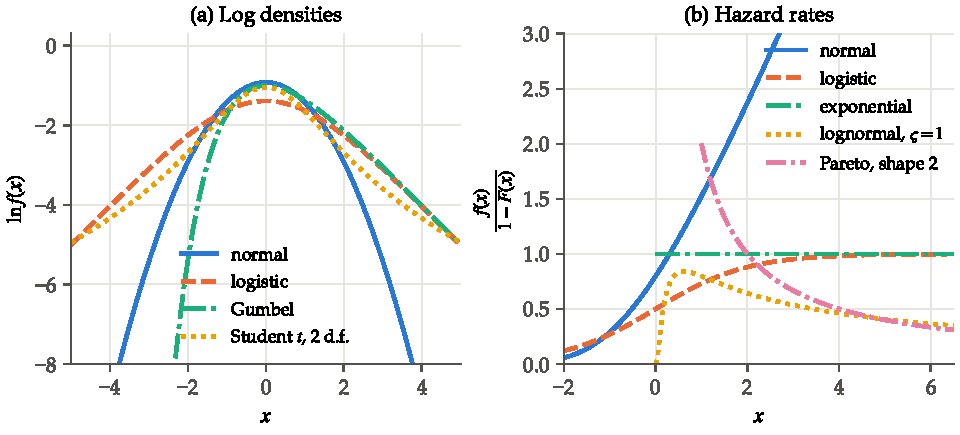
\includegraphics[width=\textwidth]{figures/appB/logconcave.pdf}
\caption{Log densities and hazard rates. Panel (a): $\ln f$ for the standard normal, standard logistic and
standard Gumbel densities, all concave, and for the Student $t$ density with two degrees of freedom, which is
convex in the tails. Panel (b): hazard rates $\frac{f(x)}{1 - F(x)}$. The normal and logistic hazards rise, the
unit exponential hazard is constant, the lognormal hazard with $\varsigma = 1$ peaks near $x = 0.62$ and then falls,
and the Pareto hazard $\frac{2}{x}$ falls.}
\label{fig:B-logconcave}
\end{figure}

\subsection{Pricing applications}\label{sec:B-lc-pricing}

\casehead{Monopoly}
Consider a single-product monopolist with constant marginal cost $c$ and differentiable demand $Q(p)$ that is
nonincreasing and positive on an interval $(c, \bar p)$, with $\bar p \leq \infty$ and $Q(p) = 0$ for $p \geq \bar p$.
Profit is $\pi(p) = (p - c)Q(p)$. Write $m(p) = -\frac{Q(p)}{Q'(p)}$ for the dollar markup that the first-order
condition supports at price $p$, the reciprocal of the semi-elasticity $-\frac{Q'}{Q}$ (\cref{ch:theory}).

\begin{proposition}[Log-concave demand and the monopoly problem]\label{prop:B-lc-monopoly}
Suppose $Q$ is log-concave on $(c, \bar p)$.
\begin{enumerate}[label=(\roman*)]
  \item Profit is log-concave on $(c, \bar p)$ and quasi-concave on $\R$, so the set of profit-maximizing prices
  is an interval.
  \item The first-order condition $p - c = m(p)$ has at most one solution in $(c, \bar p)$, and a solution is the
  global profit maximizer.
  \item Where $m$ is differentiable at the optimum, monopoly pass-through satisfies
  $\rho = \frac{1}{1 - m'(p)} \in (0, 1]$.
\end{enumerate}
If $Q$ is strictly log-concave, the maximizer is unique.
\end{proposition}

\begin{proof}
(i) On $(c, \bar p)$ profit is positive and $\ln\pi(p) = \ln(p - c) + \ln Q(p)$. Both terms are concave, so
$\ln\pi$ is concave. Outside $(c, \bar p)$ profit is nonpositive. Each upper contour set $\{p : \pi(p) \geq k\}$
with $k > 0$ is an upper contour set of the concave function $\ln\pi$, hence an interval. For $k \leq 0$ the set
contains all prices above $c$. It is an interval because profit is nondecreasing below $c$, where a higher price
shrinks both the loss per unit and the number of units sold.

(ii) Since $(\ln Q)' = \frac{Q'}{Q}$ is nonincreasing, the semi-elasticity $-\frac{Q'}{Q}$ is nondecreasing and
the markup $m(p)$ is nonincreasing where $Q' < 0$. The left side $p - c$ of the first-order condition is strictly
increasing. The two sides can cross at most once. A solution makes $(\ln\pi)'$ vanish, and a stationary point of a
concave function is a global maximizer on $(c, \bar p)$, where all positive profits are earned.

(iii) Differentiate the identity $p(c) - c = m(p(c))$ with respect to $c$:
\[
  \rho - 1 = m'(p)\rho.
\]
Solving gives $\rho = \frac{1}{1 - m'(p)}$, and $m' \leq 0$ gives $0 < \rho \leq 1$. Strict log-concavity makes $\ln\pi$
strictly concave, so the maximizer is unique.
\end{proof}

Part (iii) is the global counterpart of \cref{cor:B-passthrough-logconcave}. That corollary states that at the
monopoly price pass-through is below one if and only if $(\ln Q)'' < 0$ and above one if and only if $(\ln Q)'' > 0$. The
two statements agree because $m' = -1 + \frac{QQ''}{(Q')^2}$, so $\frac{1}{1 - m'} = \frac{1}{2 - \frac{QQ''}{(Q')^2}}$.

The proposition has a probabilistic reading. Suppose consumers have unit demand and their willingness to pay
$W$ has CDF $F_W$ and density $f_W$. Demand is $Q(p) = M[1 - F_W(p)]$ for market size $M$, and the markup is
$m(p) = \frac{1 - F_W(p)}{f_W(p)}$, the reciprocal of the hazard rate of $W$. Demand is log-concave exactly when
the survival function of $W$ is log-concave, that is, when $W$ has an increasing failure rate
(\cref{cor:B-hazard}). A log-concave density of willingness to pay suffices (\cref{prop:B-lc-cdf}). The same
object reappears as Myerson's virtual valuation in \cref{sec:B-lc-auctions}.

\casehead{Constant pass-through}
Pass-through usually varies with the level of cost. \citet{BulowPfleiderer1983} identify the demand curves for
which it does not. Let $P(q)$ be inverse demand with $P' < 0$ and curvature
$\chi(q) = -\frac{qP''(q)}{P'(q)}$, as in \eqref{eq:B-chi}. By \cref{prop:B-passthrough-monopoly}, monopoly
pass-through at output $q$ is $\rho = \frac{1}{2 - \chi(q)}$, and the second-order condition is $2 - \chi > 0$.

\begin{proposition}[Constant pass-through demands]\label{prop:B-constant-pt}
Let a monopolist with constant marginal cost face a twice continuously differentiable inverse demand with
$P' < 0$ and $2 - \chi > 0$ on an interval of outputs. Pass-through is the same at every cost in an interval of
costs if and only if inverse demand takes one of the two forms below on the corresponding interval of outputs.
\begin{enumerate}[label=(\alph*)]
  \item $P(q) = a - bq^\gamma$ with $b\gamma > 0$ and $\gamma > -1$, in which case $\rho = \frac{1}{1 + \gamma}$.
  \item $P(q) = a - b\ln q$ with $b > 0$, in which case $\rho = 1$.
\end{enumerate}
\end{proposition}

\Cref{prop:02-pt-constant} states the result in the same notation and leaves the converse as an exercise. The
proof below carries it out.

\begin{proof}
Monopoly output $q^*(c)$ is continuous and strictly decreasing, because the implicit function theorem gives
$\frac{\dd q^*}{\dd c} = \frac{1}{2P' + qP''} = \frac{1}{P'(2 - \chi)} < 0$. Hence $\rho = \frac{1}{2 - \chi(q^*(c))}$ is
constant on an interval of costs if and only if $\chi$ is constant on the image interval of outputs.

It remains to solve $qP''(q) = -\chi P'(q)$ for a constant $\chi$. Since $P' < 0$, write $-P'(q) = e^{\ell(q)}$. Then
$P'' = P'\ell'$, and the equation becomes $q\ell'(q) = -\chi$. Integrating $\ell'(q) = -\frac{\chi}{q}$ gives
$\ell(q) = -\chi\ln q + \ln K$ for a constant $K > 0$, so
\[
  P'(q) = -Kq^{-\chi}.
\]
If $\chi \neq 1$, integrate once more and set $\gamma = 1 - \chi$ and $b = \frac{K}{\gamma}$:
\[
  P(q) = a - \frac{K}{1 - \chi}q^{1 - \chi} = a - bq^\gamma,
\]
with $b\gamma = K > 0$. The second-order condition $2 - \chi > 0$ is $\gamma > -1$, and
$\rho = \frac{1}{2 - (1 - \gamma)} = \frac{1}{1 + \gamma}$. If $\chi = 1$, integrating $P' = -Kq^{-1}$ gives
$P(q) = a - K\ln q$, form (b) with $b = K$, and $\rho = \frac{1}{2 - 1} = 1$. Conversely, direct differentiation shows
that form (a) has $\chi = 1 - \gamma$ and form (b) has $\chi = 1$ at every output.
\end{proof}

The family contains the three textbook cases of \cref{ex:B-passthrough}. Linear demand is $\gamma = 1$ with
$\rho = \frac{1}{2}$. Constant-elasticity demand $P = q^{-\frac{1}{\varepsilon}}$ with $\varepsilon > 1$ is $a = 0$,
$b = -1$ and $\gamma = -\frac{1}{\varepsilon} \in (-1, 0)$, so $\rho = \frac{1}{1 - \frac{1}{\varepsilon}} = \frac{\varepsilon}{\varepsilon - 1} > 1$.
Exponential demand $Q = e^{\frac{a - p}{b}}$ is form (b) with $\rho = 1$. The family also sorts demand by
log-concavity. Since $\frac{QQ''}{(Q')^2} = \chi = 1 - \gamma$ (\cref{prop:B-passthrough-monopoly}), direct demand is strictly
log-concave when $\gamma > 0$, log-linear in form (b), and strictly log-convex when $-1 < \gamma < 0$. The ranking
of pass-through rates matches \cref{prop:B-lc-monopoly}.

\begin{example}[Power demand in prices]\label{ex:B-power-demand}
Let direct demand be $Q(p) = B(\bar p - p)^{g}$ for $p < \bar p$, with $B, g > 0$, as in \cref{tab:02-pt-examples}. Its
log is $\ln B + g\ln(\bar p - p)$, with second derivative $-\frac{g}{(\bar p - p)^2} < 0$, so demand is strictly
log-concave. Inverting $q = B(\bar p - p)^{g}$ gives
\[
  P(q) = \bar p - B^{-\frac{1}{g}}\,q^{\frac{1}{g}},
\]
which is form (a) with $a = \bar p$, $\gamma = \frac{1}{g}$ and $b = B^{-\frac{1}{g}}$. Directly, the first-order
condition $p - c = m(p)$ reads
\[
  p - c = \frac{\bar p - p}{g}.
\]
Solving gives $p = \frac{\bar p + gc}{1 + g}$, so $\rho = \frac{g}{1 + g} = \frac{1}{1 + \gamma}$, as
\cref{prop:B-constant-pt} predicts. Under a constant conduct parameter $\theta$ and flat marginal cost,
\cref{cor:B-passthrough-cases}(a) gives $\rho = \frac{1}{1 + \theta(1 - \chi)} = \frac{1}{1 + \theta\gamma} = \frac{1}{1 + \frac{\theta}{g}} = \frac{g}{g + \theta}$,
again independent of cost. This family appears in the sugar-refining application of \cref{ch:conduct}.
\end{example}

\begin{example}[Logit demand is log-concave]\label{ex:B-logit-lc}
Hold rivals' prices fixed and write single-product logit demand for product $j$ as
$s_j(p_j) = \frac{e^{\tilde\delta_j - \alpha p_j}}{\Lambda_{-j} + e^{\tilde\delta_j - \alpha p_j}}$, where $\tilde\delta_j$ is the
price-free part of mean utility and $\Lambda_{-j} = 1 + \sum_{l \neq j}e^{\delta_l}$ (\cref{sec:B-ev}).
Differentiating the log,
\[
  \frac{\dd\ln s_j}{\dd p_j} = -\alpha + \alpha s_j = -\alpha(1 - s_j),
\]
and differentiating again with $\frac{\dd s_j}{\dd p_j} = -\alpha s_j(1 - s_j)$,
\[
  \frac{\dd^2\ln s_j}{\dd p_j^2} = \alpha\frac{\dd s_j}{\dd p_j} = -\alpha^2s_j(1 - s_j) < 0.
\]
Residual demand is strictly log-concave. By \cref{prop:B-lc-monopoly}, each firm has a unique best response,
the solution of $p_j - mc_j = \frac{1}{\alpha(1 - s_j)}$ (\cref{prop:B-logit-br} gives it in closed form). Part
(iii) of the proposition puts own pass-through with rivals' prices fixed in $(0, 1]$, and
\cref{ex:B-passthrough}(iv) computes it exactly as $1 - s_j$.
\end{example}

\subsection{Aggregation and the existence of price equilibrium}\label{sec:B-caplin-nalebuff}

With several differentiated products, the existence of a pure-strategy Bertrand-Nash equilibrium requires each
firm's profit to be quasi-concave in its own price. Otherwise best responses can jump and Kakutani's theorem
fails. Demand is an aggregate over heterogeneous consumers, so the question is which primitives make aggregate
demand concave enough. \citet{CaplinNalebuff1991} answer it with \cref{thm:B-prekopa-borell}. \Cref{sec:04-cn}
proves their theorems and discusses their economic coverage. This subsection restates the argument as an
application of $\varrho$-concavity and refers to those proofs.

\casehead{Setting}
There are $J$ firms. Firm $j$ sells one product with fixed characteristics $x_j$ at constant marginal cost
$c_j$, and firms set prices simultaneously. Each consumer has income $y > 0$ and buys one unit of exactly one
product, consuming $z = y - p_j$ of a numeraire. Consumers differ by a type $\nu \in \R^L$ with density $f$ and
convex support $B$. The dimension $L$ of the type space is local to this subsection. \citet{CaplinNalebuff1991}
impose two assumptions.

\begin{assumption}[A1, preferences linear in the type]\label{ass:B-cn-a1}
Utility is $U(\nu, x, z) = \sum_{l=1}^L \nu_l t_l(x) + g(z)t_{L+1}(x) + t_{L+2}(x)$, where $t : X \to \R^{L+2}$ maps
characteristics into benefits, $g$ is strictly increasing and concave, and $t_{L+1}(x) > 0$.
\end{assumption}

\begin{assumption}[A2, concavity of the type density]\label{ass:B-cn-a2}
The density $f$ is $\varrho$-concave with $\varrho = -\frac{1}{L + 1}$, on a convex support with positive volume.
\end{assumption}

All consumers agree on the benefits $t_l(x)$ that a product delivers and differ in the weights $\nu_l$ they place on
them. By \cref{lem:B-rho-hierarchy}, every log-concave density satisfies A2. A2 also admits the multivariate
Cauchy, Pareto, F and Student $t$ distributions under restrictions on their parameters, for the Student $t$ at
least one degree of freedom \citep[Section 3, p.~6]{CaplinNalebuff1991}. A1 covers
characteristics models, quadratic transport costs, vertical differentiation, and logit, probit and random
coefficients models with a common price coefficient. It excludes Hotelling's linear transport costs, whose
demand is discontinuous.

\casehead{Demand as the probability of a set}
Fix rivals' prices $p_{-j}$. Let $\mathcal{A}_j(p_j)$ be the set of types that weakly prefer product $j$ at price
$p_j$ to every rival,
\[
  \mathcal{A}_j(p_j) = \bigl\{\nu : \Delta_k(\nu, p_j) \geq 0 \text{ for all } k \neq j\bigr\},
  \qquad \Delta_k(\nu, p_j) = U(\nu, x_j, y - p_j) - U(\nu, x_k, y - p_k)\text{.}
\]

Ties occur on hyperplanes of types when products are distinct, so they have probability zero. Demand is
\begin{equation}\label{eq:B-cn-demand}
  D_j(p_j) = \int_{\mathcal{A}_j(p_j)} f(\nu)\,\dd\nu,
\end{equation}
which is the demand function of \citet[Section 4]{CaplinNalebuff1991}, written with the set of buyers instead of
reservation prices. Given rivals' prices, firm $j$ is a monopolist facing a population of reservation prices.

\begin{lemma}[Buyer sets are Minkowski-concave]\label{lem:B-cn-minkowski}
Under A1, for any prices $p_0$, $p_1$ and $\lambda \in [0, 1]$, with $p_\lambda = \lambda p_0 + (1 - \lambda)p_1$,
\[
  \mathcal{A}_j(p_\lambda) \supseteq \lambda\mathcal{A}_j(p_0) + (1 - \lambda)\mathcal{A}_j(p_1).
\]
\end{lemma}

The proof of \cref{thm:04-cn-demand} establishes this inclusion. It averages the preference inequalities of
types $\nu_0$ and $\nu_1$, which A1 makes linear in the type, and uses concavity of $g$ for the price term.

\begin{theorem}[Aggregation, \citealp{CaplinNalebuff1991}, Section 4]\label{thm:B-cn-aggregation}
Assume A1, distinct products and a $\varrho$-concave type density with $\varrho \geq -\frac{1}{L}$. Then each firm's demand
$D_j(p_j)$ is $\varrho^*$-concave in its own price, with $\varrho^* = \frac{\varrho}{1 + L\varrho}$, on the interval of prices
where it is positive.
\end{theorem}

This is \cref{thm:04-cn-demand}. For prices $p_0$ and $p_1$ with positive demand, \cref{lem:B-cn-minkowski},
monotonicity of the integral and \cref{thm:B-prekopa-borell} give
\[
  D_j(p_\lambda) \geq \int_{\lambda\mathcal{A}_j(p_0) + (1 - \lambda)\mathcal{A}_j(p_1)} f(\nu)\,\dd\nu
  \geq \mathcal{M}_{\varrho^*}\bigl(D_j(p_0), D_j(p_1); \lambda\bigr).
\]
The bound is tight (\cref{ex:04-cn-simplex}). With types uniform on the unit simplex and reservation prices
$1 - \sum_l\nu_l$, demand is $D(p) = (1 - p)^L$, which is $\frac{1}{L}$-concave and no more.

\casehead{Quasi-concave profit}
The second step turns concavity of demand into quasi-concavity of profit.

\begin{proposition}[Convex reciprocal demand gives quasi-concave profit]\label{prop:B-cn-quasiconcave}
Let marginal cost $c$ be constant and let demand $D$ be nonincreasing, positive on an interval $(-\infty, \bar p)$
and zero above it. If $\frac{1}{D}$ is convex on $(-\infty, \bar p)$, then profit $\pi(p) = (p - c)D(p)$ is
quasi-concave.
\end{proposition}

\Cref{lem:04-recip} proves the result by contradiction, following \citet[p.~29]{CaplinNalebuff1991}. A direct
argument uses upper contour sets. For $k > 0$ and prices in $(c, \bar p)$, $\pi(p) \geq k$ holds if and only if
$p - c - \frac{k}{D(p)} \geq 0$. The left side is linear minus a convex function, hence concave, so its upper
contour set is an interval. For $k \leq 0$ the set contains every price above $c$, and profit is nondecreasing
below $c$.

For strictly decreasing, twice differentiable demand, $\frac{1}{D}$ is convex if and only if revenue $qP(q)$ is
concave in quantity (\cref{sec:04-existence-demand} gives the computation). \citet[Section 5]{CaplinNalebuff1991}
note that concave revenue is equivalent to quasi-concavity of profit for every convex cost function. The condition is therefore as weak as possible when costs are unrestricted. In the language of
\cref{def:B-rhoconcave}, $\frac{1}{D}$ convex means that $D$ is $(-1)$-concave. \Cref{thm:B-cn-aggregation}
delivers this when $\varrho^* \geq -1$. Solving $\frac{\varrho}{1 + L\varrho} = -1$ step by step,
\begin{align*}
  \varrho &= -(1 + L\varrho),\\
  \varrho(1 + L) &= -1,\\
  \varrho &= -\frac{1}{L + 1}.
\end{align*}
Because $\varrho^*$ is increasing in $\varrho$ and $-\frac{1}{L + 1} > -\frac{1}{L}$, every density that satisfies A2 yields
$\varrho^* \geq -1$, hence $(-1)$-concave demand by \cref{lem:B-rho-hierarchy}, hence quasi-concave profit. This
is why A2 has the exponent $-\frac{1}{L + 1}$. The same calculation shows why earlier work that assumed concave
demand was confined to special cases. Concave demand needs $\varrho^* = 1$, which requires $\varrho = \infty$ and
$L = 1$, a uniform distribution of types on a line \citep[Section 5]{CaplinNalebuff1991}.

\begin{theorem}[Existence, \citealp{CaplinNalebuff1991}, Section 5]\label{thm:B-cn-existence}
Under A1 and A2, for any number of firms and any products, a pure-strategy Bertrand-Nash equilibrium exists.
\end{theorem}

\Cref{thm:04-cn-existence} proves the theorem. With distinct products, it restricts each firm to prices in
$[c_j, y]$, where profits are continuous. Quasi-concavity in own price makes each best-response set an interval,
and Kakutani's theorem (\cref{thm:B-kakutani}) gives a fixed point. Equivalent products and costs above income
are handled separately.

\casehead{Uniqueness and log-supermodularity}
\citet[Section 6]{CaplinNalebuff1991} prove uniqueness under differentiability in three cases.
\begin{enumerate}[label=(\alph*)]
  \item Duopoly with a log-concave type density, in any dimension.
  \item Any number of firms in a one-dimensional market with a log-concave density, given the set of active firms.
  \item The logit model.
\end{enumerate}
The tool is the dominant-diagonal condition
$\bigl|\frac{\partial^2\pi_j}{\partial p_j^2}\bigr| > \sum_{k \neq j}\bigl|\frac{\partial^2\pi_j}{\partial p_j\,\partial p_k}\bigr|$, which
allows at most one equilibrium among a given set of active firms \citep{Friedman1977}
(\cref{prop:B-dd-uniqueness}). In all three cases the pricing game is also log-supermodular, a property
studied in \cref{sec:B-supermodular-games}.

The logit case was checked in \cref{sec:B-equilibrium}. There the log first-order conditions
$\frac{\partial\ln\pi_j}{\partial p_j} = \frac{1}{p_j - c_j} - \alpha(1 - s_j) = 0$ satisfy the dominant-diagonal condition on
the set of prices above cost. On the best response, the implicit function theorem turns the same derivatives into
the slopes $\frac{\partial BR_j}{\partial p_k} = \frac{s_js_k}{1 - s_j} > 0$, whose row sums are below one
(\cref{prop:B-logit-br-contraction}). Best responses slope up, so logit prices are strategic complements.

Log-supermodularity combined with uniqueness has strong consequences \citep{MilgromRoberts1990}. Caplin and
Nalebuff list four.
\begin{enumerate}[label=(\arabic*)]
  \item There are no other equilibria in mixed or correlated strategies.
  \item The equilibrium is globally stable under best-response dynamics, fictitious play and Bayesian learning.
  \item The game is dominance solvable.
  \item Any change that raises some firm's marginal return to price raises every firm's equilibrium price.
\end{enumerate}
A cost increase for one firm, for instance, raises all prices (\cref{ex:B-logit-cost}).

The theorem has limits. It assumes unit demand, single-product firms and fixed products. Multiproduct logit
pricing is unique by a different argument (\cref{sec:B-fixedpoint}). A random price coefficient fits A1 only
after utility is divided by it, and A2 must then hold for the distribution of the resulting ratios, which can fail
(\cref{sec:04-cn}).

Random price coefficients are often lognormal in random coefficients demand models, so the lognormal deserves a
check. \citet[Section 3, p.~6]{CaplinNalebuff1991} note that A2 survives the truncation of a density to a convex
support but not other transformations. They give the lognormal as a distribution that fails A2. The failure
depends on the dispersion. With $L = 1$, A2 requires $f^{-\frac{1}{2}}$ to be convex. Let $\ln\nu \sim N(m,
\varsigma^2)$ and write $t = \ln\nu$. Up to a positive constant, $f(\nu)^{-\frac{1}{2}} = e^{g(t)}$ with
\[
  g(t) = \frac{t}{2} + \frac{(t - m)^2}{4\varsigma^2}.
\]
Since $\frac{\dd}{\dd\nu} = \frac{1}{\nu}\frac{\dd}{\dd t}$, differentiating twice gives
\[
  \frac{\dd^2}{\dd\nu^2}e^{g(t)} = \frac{e^{g(t)}}{\nu^2}\bigl[g'(t)^2 - g'(t) + g''(t)\bigr]
  = \frac{e^{g(t)}}{\nu^2}\Bigl[\Bigl(g'(t) - \frac{1}{2}\Bigr)^2 - \frac{1}{4} + \frac{1}{2\varsigma^2}\Bigr].
\]
The derivative $g'(t) = \frac{1}{2} + \frac{t - m}{2\varsigma^2}$ takes every real value, so the bracket is nonnegative
everywhere exactly when $\frac{1}{2\varsigma^2} \geq \frac{1}{4}$, that is, when $\varsigma^2 \leq 2$. A
one-dimensional lognormal therefore satisfies A2 for moderate dispersion and fails it for large dispersion. Its
density is never log-concave (\cref{tab:B-logconcave}), so here A2 is a real gain over log-concavity.

\subsection{Auction applications}\label{sec:B-lc-auctions}

Hazard rates and reverse hazard rates are the natural objects in auction theory. The hazard rate governs the
seller's trade-off between price and probability of sale. The reverse hazard rate governs a bidder's trade-off
between the margin and the probability of winning. In this subsection a bidder's value has CDF $F$ with density
$f > 0$ on $[\underline v, \bar v]$, and the seller values the object at $v_0$.

\begin{proposition}[Myerson regularity]\label{prop:B-regular}
If the hazard rate $\frac{f}{1 - F}$ is nondecreasing, the virtual valuation
$\psi(v) = v - \frac{1 - F(v)}{f(v)}$ is strictly increasing, so $F$ is regular. A log-concave density suffices.
\end{proposition}

\begin{proof}
The term $\frac{1 - F}{f}$ is the reciprocal of a nondecreasing positive function, so it is nonincreasing. Then
$\psi$ is the sum of the strictly increasing function $v$ and the nondecreasing function $-\frac{1 - F}{f}$. A
log-concave density has a nondecreasing hazard rate by \cref{cor:B-hazard}.
\end{proof}

Regularity makes the optimal reserve price the unique solution of $r^* - \frac{1 - F(r^*)}{f(r^*)} = v_0$, because
the left side is strictly increasing \citep{Myerson1981}. For values uniform on $[0, 1]$,
$\psi(v) = v - (1 - v) = 2v - 1$ and $r^* = \frac{1 + v_0}{2}$. For exponential values with rate $\lambda$,
$\psi(v) = v - \frac{1}{\lambda}$ and $r^* = v_0 + \frac{1}{\lambda}$. The seller's problem with one bidder is the monopoly
problem of \cref{prop:B-lc-monopoly} with willingness to pay $V$ and cost $v_0$. \Cref{cor:14-optimal-reserve} in
\cref{ch:auction-theory} gives the general result.

Consider a symmetric first-price auction with independent private values and $N$ bidders. A bidder who bids $b$
must have value $\xi(b) = b + \frac{G(b)}{(N - 1)g(b)}$ \citep{GuerrePerrigneVuong2000}. Here $G$ and $g$ are the
distribution and density of equilibrium bids. \citet[Theorem 1]{GuerrePerrigneVuong2000} write $I$ for the number of
bidders. They show that an observed bid distribution is rationalized by some value distribution if and only if
bids are i.i.d.\ and $\xi$ is strictly increasing with a differentiable inverse. The second requirement is their
condition C2.

\begin{proposition}[Log-concave bids satisfy the monotonicity condition]\label{prop:B-gpv-monotone}
Let $G$ have a positive differentiable density $g$ on $[\underline b, \bar b]$. If $G$ is log-concave, then
$\xi(b) = b + \frac{G(b)}{(N - 1)g(b)}$ is strictly increasing. More generally, $\xi$ is strictly increasing if and
only if $\frac{g}{G^N}$ is strictly decreasing.
\end{proposition}

\begin{proof}
If $G$ is log-concave, the reverse hazard rate $\frac{g}{G}$ is nonincreasing (\cref{cor:B-hazard}), so
$\frac{G}{g}$ is nondecreasing. Then $\xi$ is the sum of the strictly increasing function $b$ and a nondecreasing
function. For the general statement, differentiate $\xi$ by the quotient rule:
\[
  \xi'(b) = 1 + \frac{g(b)^2 - G(b)g'(b)}{(N - 1)g(b)^2} = \frac{Ng(b)^2 - G(b)g'(b)}{(N - 1)g(b)^2}.
\]
Differentiating $\frac{g}{G^N}$ gives
\[
  \frac{\dd}{\dd b}\left(\frac{g}{G^N}\right) = \frac{g'G^N - NG^{N-1}g^2}{G^{2N}} = -\frac{Ng^2 - Gg'}{G^{N+1}}.
\]
The two derivatives have opposite signs. Hence $\xi' > 0$ exactly when $\frac{g}{G^N}$ is strictly decreasing
\citep[p.~530 and footnote 6]{GuerrePerrigneVuong2000}.
\end{proof}

Log-concavity is sufficient for condition C2 and far from necessary. A violation needs a bid density that
falls steeply relative to $G$. \citet[p.~530]{GuerrePerrigneVuong2000} give the example
$G(b) = \bigl(\frac{b}{5 - 4b}\bigr)^{\frac{1}{5}}$ on $[0, 1]$ with $N = 2$, whose density has a deep U shape. Here
$\frac{\dd\ln G}{\dd b} = \frac{1}{5}\bigl(\frac{1}{b} + \frac{4}{5 - 4b}\bigr) = \frac{1}{b(5 - 4b)}$, so
\[
  \xi(b) = b + b(5 - 4b) = 6b - 4b^2,
\]
which decreases for $b > \frac{3}{4}$. No independent private values model generates these bids. The
identification argument is developed in \cref{ch:auction-empirics}.

Reverse hazard rates also compare bidders. In an asymmetric auction, a strong bidder's value distribution $F_s$
and a weak bidder's $F_w$ are typically ranked by the reverse hazard rate. The ranking implies first-order
dominance.

\begin{proposition}[Reverse hazard rate dominance implies first-order dominance]\label{prop:B-rh-fosd}
Let $F_s$ and $F_w$ have positive densities $f_s$ and $f_w$ on a common support $[\underline v, \bar v]$. If
$\frac{f_s(v)}{F_s(v)} \geq \frac{f_w(v)}{F_w(v)}$ for all $v \in (\underline v, \bar v)$, then $F_s(v) \leq F_w(v)$ for all $v$.
\end{proposition}

\begin{proof}
Since $\frac{f}{F} = \frac{\dd}{\dd v}\ln F$, the hypothesis says
\[
  \frac{\dd}{\dd v}\ln\frac{F_s(v)}{F_w(v)} = \frac{f_s(v)}{F_s(v)} - \frac{f_w(v)}{F_w(v)} \geq 0,
\]
so the ratio $\frac{F_s}{F_w}$ is nondecreasing on $(\underline v, \bar v)$. Its limit at $\bar v$ is
$\frac{F_s(\bar v)}{F_w(\bar v)} = 1$. Hence $\frac{F_s(v)}{F_w(v)} \leq 1$, that is, $F_s(v) \leq F_w(v)$, for every
$v \in (\underline v, \bar v)$. At the endpoints both CDFs coincide.
\end{proof}

\Cref{sec:14-asym} extends the result to supports with different upper ends. The reverse hazard rate order is
the assumption under which \citet{MaskinRiley2000} sign equilibrium behavior in asymmetric first-price
auctions. The strong bidder shades its bid more, yet its bids are stochastically higher. The weak bidder sometimes
wins although its value is lower. \Cref{sec:B-stochastic-orders} places the order in the full chain of
stochastic orders.

\section{Supermodularity, monotone comparative statics and affiliation}\label{sec:B-supermod}

The implicit function theorem signs comparative statics through derivatives and second-order conditions
(\cref{prop:B-cs-optimum}). Many economic problems lack the smoothness or the concavity that this route needs.
Choices may be discrete, maximizers may jump, and profit functions may have several local peaks. Lattice
methods sign comparative statics from a single property, complementarity between the choice and the parameter,
and they extend to games and to probability. This section develops the order-theoretic tools and their uses in
oligopoly pricing, the vertical model and auctions. It ends with affiliation, the form of positive dependence that
auction theory uses.

\subsection{Lattices and supermodular functions}\label{sec:B-lattice}

We order $\R^k$ componentwise: $x \geq y$ means $x_l \geq y_l$ for every $l$. This is a \emph{partial order}, since two
vectors need not be comparable. The \emph{join} $x \vee y$ and the \emph{meet} $x \wedge y$ are the componentwise
maximum and minimum,
\[
  (x \vee y)_l = \max\{x_l, y_l\}, \qquad (x \wedge y)_l = \min\{x_l, y_l\}.
\]

\begin{definition}[Lattices]\label{def:B-lattice}
A set $X \subseteq \R^k$ is a \emph{lattice} (a sublattice of $\R^k$) if $x \vee y \in X$ and $x \wedge y \in X$ whenever
$x, y \in X$. A lattice is \emph{complete} if every nonempty subset has a supremum and an infimum in $X$.
\end{definition}

The whole space $\R^k$ and every product of intervals are lattices. A compact product of closed intervals is a
complete lattice. The set $\{x \in \R^2 : x_1 \leq x_2\}$ is a lattice, because the componentwise maximum and minimum
of two points with $x_1 \leq x_2$ inherit the inequality. The set $\{x \in \R^2 : x_1 + x_2 \leq 1\}$ is convex but not a
lattice: $(1, 0)$ and $(0, 1)$ belong to it, while their join $(1, 1)$ does not. Lattices are about order, convex
sets about averages, and the two notions are independent.

\begin{definition}[Supermodularity and increasing differences]\label{def:B-supermodular}
Let $X$ be a lattice and $A$ a partially ordered set of parameters.
\begin{enumerate}[label=(\roman*)]
  \item A function $g : X \to \R$ is \emph{supermodular} if $g(x \vee y) + g(x \wedge y) \geq g(x) + g(y)$ for all
  $x, y \in X$.
  \item A function $g : X \times A \to \R$ has \emph{increasing differences} in $(x, a)$ if, for all $x' \geq x$, the
  difference $g(x', a) - g(x, a)$ is nondecreasing in $a$. It has \emph{strictly increasing differences} if the
  difference is strictly increasing in $a$ whenever $x' > x$.
  \item A positive function $g$ is \emph{log-supermodular} if $\ln g$ is supermodular.
\end{enumerate}
\end{definition}

For two variables the two notions coincide. Take $x = (x_1', x_2)$ and $y = (x_1, x_2')$ with $x_1' \geq x_1$ and
$x_2' \geq x_2$. Then $x \vee y = (x_1', x_2')$ and $x \wedge y = (x_1, x_2)$, and supermodularity reads
\[
  g(x_1', x_2') - g(x_1, x_2') \geq g(x_1', x_2) - g(x_1, x_2),
\]
which says that the gain from raising the first variable is larger when the second is larger. Supermodularity is
the formal statement of complementarity. Ordered pairs impose nothing, because then $\{x \vee y, x \wedge y\} = \{x, y\}$.
For smooth functions on products of intervals there is a derivative test.

\begin{proposition}[Smooth test, \citealp{Topkis1978}]\label{prop:B-smooth-supermod}
Let $X = \prod_{l=1}^k I_l$ be a product of open intervals and let $g : X \to \R$ be twice continuously
differentiable. Then $g$ is supermodular if and only if $\frac{\partial^2g}{\partial x_l\,\partial x_m} \geq 0$ for all
$l \neq m$ at every point of $X$.
\end{proposition}

\begin{proof}
Suppose the cross partials are nonnegative and take $x, y \in X$. Let $z = x \wedge y$, $u = x - z \geq 0$ and
$w = y - z \geq 0$. A coordinate $l$ has $u_l > 0$ only if $x_l > y_l$, and $w_l > 0$ only if $y_l > x_l$, so $u$ and $w$
have disjoint supports. Moreover $x = z + u$, $y = z + w$ and $x \vee y = z + u + w$. We must show
\[
  g(z + u + w) - g(z + w) - g(z + u) + g(z) \geq 0\text{.}
\]
By the fundamental theorem of calculus along the segment from $z$ to $z + w$,
\[
  g(z + u + w) - g(z + w) - g(z + u) + g(z) = \int_0^1 \sum_m w_m\left[\frac{\partial g}{\partial x_m}(z + u + tw) - \frac{\partial g}{\partial x_m}(z + tw)\right]\dd t\text{.}
\]

Applying the theorem again along the segment from $z + tw$ to $z + u + tw$,
\[
  g(z + u + w) - g(z + w) - g(z + u) + g(z) = \int_0^1\!\!\int_0^1 \sum_m\sum_l w_mu_l\,\frac{\partial^2g}{\partial x_l\,\partial x_m}(z + su + tw)\,\dd s\,\dd t\text{.}
\]

Every term with $w_mu_l \neq 0$ has $l \neq m$ by disjointness, so it multiplies a nonnegative cross partial by a
nonnegative weight. The integral is nonnegative.

Conversely, suppose $g$ is supermodular and fix $l \neq m$, a point $x$, and small $\epsilon, \eta > 0$. Apply the
two-variable inequality above to coordinates $l$ and $m$ with the others held at $x$:
\[
  g(x + \epsilon e_l + \eta e_m) - g(x + \eta e_m) - g(x + \epsilon e_l) + g(x) \geq 0,
\]
where $e_l$ is the $l$-th unit vector. Divide by $\epsilon\eta$ and let $\epsilon, \eta \to 0$. By the double-integral
representation and continuity of the cross partial, the limit is $\frac{\partial^2g}{\partial x_l\,\partial x_m}(x) \geq 0$.
\end{proof}

The proposition applies to $\ln g$ as well. A positive $C^2$ function is log-supermodular if and only if
$\frac{\partial^2\ln g}{\partial x_l\,\partial x_m} \geq 0$ for $l \neq m$. Products of log-supermodular functions are
log-supermodular, because logs add. The same test applied to a function of $(x, a)$ with $x$ and $a$ scalars shows
that a $C^2$ function has increasing differences if and only if $\frac{\partial^2g}{\partial x\,\partial a} \geq 0$.

\subsection{Monotone comparative statics}\label{sec:B-topkis}

To compare sets of maximizers we need an order on sets.

\begin{definition}[Strong set order]\label{def:B-sso}
For subsets $S, S'$ of a lattice, $S'$ is higher than $S$ in the \emph{strong set order}, written $S' \geq_S S$, if
$x \vee x' \in S'$ and $x \wedge x' \in S$ for all $x \in S$ and $x' \in S'$.
\end{definition}

For compact intervals of $\R$, $S' \geq_S S$ means that $\max S' \geq \max S$ and $\min S' \geq \min S$. For general
compact subsets of $\R$ these inequalities are necessary but not sufficient. The sets $S = \{0, 2\}$ and $S' = \{1, 3\}$
satisfy both, yet $2 \vee 1 = 2 \notin S'$. For singletons it means $x' \geq x$.

\begin{theorem}[Topkis]\label{thm:B-topkis}
Let $X$ be a lattice, $A$ a partially ordered set, and $g : X \times A \to \R$ supermodular in $x$ for each $a$ and with
increasing differences in $(x, a)$. Let $M(a) = \argmax_{x \in X}g(x, a)$. If $a' \geq a$, then $M(a') \geq_S M(a)$. In
particular, the largest and smallest maximizers, when they exist, are nondecreasing in $a$ \citep{Topkis1978}.
\end{theorem}

\begin{proof}
Let $a' \geq a$, $x \in M(a)$ and $x' \in M(a')$. Both $x \vee x'$ and $x \wedge x'$ lie in $X$. Optimality of $x'$ at $a'$
and of $x$ at $a$ gives
\begin{align}
  g(x', a') &\geq g(x \vee x', a'), \label{eq:B-topkis-1}\\
  g(x, a) &\geq g(x \wedge x', a). \label{eq:B-topkis-2}
\end{align}
Supermodularity in $x$ at $a$, rearranged, and then \eqref{eq:B-topkis-2} give
\begin{equation}\label{eq:B-topkis-3}
  g(x \vee x', a) - g(x', a) \geq g(x, a) - g(x \wedge x', a) \geq 0.
\end{equation}
Since $x \vee x' \geq x'$ and $a' \geq a$, increasing differences give
\begin{equation}\label{eq:B-topkis-4}
  g(x \vee x', a') - g(x', a') \geq g(x \vee x', a) - g(x', a).
\end{equation}
Chaining \eqref{eq:B-topkis-4} and \eqref{eq:B-topkis-3}, $g(x \vee x', a') \geq g(x', a')$. With
\eqref{eq:B-topkis-1} this holds with equality, so $x \vee x' \in M(a')$. The left side of \eqref{eq:B-topkis-4} is
then zero, so every term in the chain is zero. In particular $g(x, a) = g(x \wedge x', a)$, and $x \wedge x' \in M(a)$.
\end{proof}

With strictly increasing differences and a scalar choice, every selection from the argmax is nondecreasing. To
see this, suppose $a' > a$, $x \in M(a)$, $x' \in M(a')$ and $x > x'$. Strictly increasing differences and optimality of $x$
at $a$ give $g(x, a') - g(x', a') > g(x, a) - g(x', a) \geq 0$, which contradicts optimality of $x'$ at $a'$.

Compare the theorem with \cref{prop:B-cs-optimum}. The implicit function theorem gives
$\frac{\dd x^*}{\dd a} = -\frac{g_{xa}}{g_{xx}}$, whose sign is that of $g_{xa}$ under a strict second-order condition.
Topkis's theorem reaches the qualitative conclusion from $g_{xa} \geq 0$ alone. It needs no concavity, no
differentiability in $x$, no interior solution and no uniqueness, and the choice set may be discrete. It is silent
on magnitudes, which still require derivatives.

The conditions of \cref{thm:B-topkis} are cardinal: a monotone transformation of $g$ can destroy increasing
differences without changing any argmax. \citet{MilgromShannon1994} found the ordinal conditions. A function
$g : X \to \R$ is \emph{quasi-supermodular} if $g(x) \geq g(x \wedge y)$ implies $g(x \vee y) \geq g(y)$, and the same holds
with strict inequalities. A function $g(x, a)$ satisfies the \emph{single crossing property} in $(x, a)$ if, for
$x' > x$ and $a' > a$, $g(x', a) \geq g(x, a)$ implies $g(x', a') \geq g(x, a')$, and $g(x', a) > g(x, a)$ implies
$g(x', a') > g(x, a')$. A gain from a higher choice at a low parameter persists at a higher parameter.

\begin{theorem}[\citealp{MilgromShannon1994}]\label{thm:B-milgrom-shannon}
Let $X$ be a lattice and $g : X \times A \to \R$. The following statements are equivalent.
\begin{enumerate}[label=(\alph*)]
  \item The set $\argmax_{x \in S}g(x, a)$ is nondecreasing in $(a, S)$ in the strong set order, over all sublattices
  $S \subseteq X$.
  \item The function $g$ is quasi-supermodular in $x$ and satisfies the single crossing property in $(x, a)$.
\end{enumerate}
\end{theorem}

Both conditions are preserved by strictly increasing transformations of $g$. A positive log-supermodular
function satisfies them. Indeed, if $\ln g$ has increasing differences, the ratio $\frac{g(x', a)}{g(x, a)}$ is
nondecreasing in $a$ for $x' \geq x$. If it is at least one at $a$, it is at least one at $a' > a$, which is single
crossing. This is why log-supermodularity, a cardinal condition on $\ln g$, has ordinal consequences for $g$.

\begin{example}[Monopoly price rises with cost for any demand]\label{ex:B-topkis-monopoly}
Let demand $Q(p)$ be any nonincreasing function on a price set $X = [0, \bar p]$, and let profit be
$\pi(p, c) = (p - c)Q(p)$. For $p' > p$,
\[
  \pi(p', c) - \pi(p, c) = p'Q(p') - pQ(p) - c\bigl[Q(p') - Q(p)\bigr].
\]
The bracket is nonpositive, so the difference is nondecreasing in $c$. Profit has increasing differences in
$(p, c)$, and by \cref{thm:B-topkis} the largest and smallest optimal prices are nondecreasing in marginal cost.
If $Q$ is strictly decreasing the differences are strictly increasing, and every selection of optimal prices is
nondecreasing. No curvature, concavity, continuity or differentiability of demand is used. On prices above cost,
the same conclusion follows from log-supermodularity, since
$\frac{\partial^2}{\partial p\,\partial c}\ln[(p - c)Q(p)] = \frac{\partial^2}{\partial p\,\partial c}\ln(p - c) = \frac{1}{(p - c)^2} > 0$.
The direction of pass-through is thus a free result, while its size, $\rho = \frac{1}{2 - \chi}$, depends on demand
curvature (\cref{sec:B-passthrough}).
\end{example}

\begin{example}[Sorting in the vertical model]\label{ex:B-vertical-sorting}
In the vertical model consumer $i$ obtains $u_{ij} = \delta_j - \nu_ip_j$ from product $j$, with $\nu_i > 0$ the price
sensitivity and the outside good at $\delta_0 = p_0 = 0$ (\cref{sec:06-vertical}). Index the products with positive
sales by price, $0 = p_0 < p_1 < \dots < p_J$, so that qualities rise in the same order. For $k > j$,
\[
  u_{ij} - u_{ik} = (\delta_j - \delta_k) + \nu_i(p_k - p_j),
\]
which is strictly increasing in $\nu_i$. This is the \emph{single crossing property} of the vertical model. As
functions of $\nu$, the utility lines of two products cross at most once, and the cheaper product wins for the
more price-sensitive consumers. In lattice terms, $u(j, \nu) = \delta_j - \nu p_j$ has strictly decreasing differences
in $(j, \nu)$, so by \cref{thm:B-topkis} applied with $-\nu$ as the parameter, the chosen product is nonincreasing in $\nu$.

Single crossing also explains why a consumer need compare product $j$ only with its two neighbors. Let
$\bar\nu_j = \frac{\delta_j - \delta_{j-1}}{p_j - p_{j-1}}$ be the type indifferent between $j - 1$ and $j$, and suppose the cutoffs
are strictly decreasing, $\bar\nu_1 > \bar\nu_2 > \dots > \bar\nu_J > 0$, as they are when every product sells. A
consumer prefers $j$ to $j + 1$ if and only if $\nu_i > \bar\nu_{j+1}$, and $j$ to $j - 1$ if and only if
$\nu_i < \bar\nu_j$. Suppose both hold. Then $\nu_i > \bar\nu_{j+1} > \bar\nu_{j+2}$, so she also prefers $j + 1$ to $j + 2$.
Transitivity gives $j \succ j + 2$, and induction on $k$ gives $j \succ k$ for all $k > j$. Symmetrically,
$\nu_i < \bar\nu_j < \bar\nu_{j-1}$ gives $j - 1 \succ j - 2$, hence $j \succ j - 2$ and, by induction, $j \succ k$ for all $k < j$.
With the conventions $\bar\nu_0 = \infty$ and $\bar\nu_{J+1} = 0$, the consumer chooses $j$ exactly when
$\bar\nu_{j+1} < \nu_i < \bar\nu_j$.
\end{example}

\begin{example}[Cournot best responses without concavity]\label{ex:B-cournot-topkis}
In a homogeneous-good Cournot market, firm $i$'s profit is $\pi_i(q_i, Q_{-i}) = q_iP(q_i + Q_{-i}) - C_i(q_i)$, where
$Q_{-i}$ is rivals' total output. \Cref{ex:B-cournot-br} computed the slope of the best response by the implicit
function theorem, under a strict second-order condition. The lattice argument needs only the cross partial,
\[
  \frac{\partial^2\pi_i}{\partial q_i\,\partial Q_{-i}} = P'(Q) + q_iP''(Q).
\]
If $P' + q_iP'' \leq 0$ on the relevant domain, profit has decreasing differences in $(q_i, Q_{-i})$, which are
increasing differences in $(q_i, -Q_{-i})$. By \cref{thm:B-topkis}, the extremal best responses are nonincreasing in
rivals' output. Neither concavity of profit in $q_i$ nor convexity of cost is needed, and the best response may be a
correspondence. \Cref{sec:B-strategic} shows that the sign of $P' + q_iP''$ can reverse.
\end{example}

\subsection{Strategic substitutes and complements}\label{sec:B-strategic}

\citet{BulowGeanakoplosKlemperer1985} sort competition by the sign of a single cross partial. Orient each
firm's strategic variable so that a higher value is more aggressive: quantities, advertising, or the negative of
a price.

\begin{definition}[Strategic substitutes and complements]\label{def:B-strategic}
Firm $B$ regards the products as \emph{strategic substitutes} if a more aggressive action by firm $A$ lowers $B$'s
marginal profit, that is, $\frac{\partial^2\pi_B}{\partial S_B\,\partial S_A} < 0$. It regards them as \emph{strategic
complements} if the cross partial is positive \citep[p.~494]{BulowGeanakoplosKlemperer1985}.
\end{definition}

The definition concerns marginal profit. Ordinary substitutes and complements concern the level of profit, the
sign of $\frac{\partial\pi_B}{\partial S_A}$. Under strict concavity in own action, the implicit function theorem gives
the slope of $B$'s best response (reaction function) $BR_B$,
\[
  \frac{\dd BR_B}{\dd S_A} = -\left(\frac{\partial^2\pi_B}{\partial S_B^2}\right)^{-1}\frac{\partial^2\pi_B}{\partial S_B\,\partial S_A}\text{.}
\]
Reaction curves therefore slope down under strategic substitutes and up under strategic complements. When prices are
the strategic variables, $S = -p$ and $\frac{\partial^2\pi_B}{\partial(-p_B)\,\partial(-p_A)} = \frac{\partial^2\pi_B}{\partial p_B\,\partial p_A}$, so
prices are strategic complements when $\frac{\partial^2\pi_B}{\partial p_B\,\partial p_A} > 0$.

\begin{example}[Multimarket contact and the sign of the strategic effect]\label{ex:B-bgk}
\citet[pp.~492--495]{BulowGeanakoplosKlemperer1985} study a firm $A$ that is a monopolist in market 1 and a duopolist
with firm $B$ in market 2. The strategic variables are $S_1^A$, $S_2^A$ and $S_2^B$. A shock $Z$ raises $A$'s marginal
profit in market 1, so $\pi^A = R_1^A(S_1^A) + R_2^A(S_2^A, S_2^B) - C^A(S_1^A, S_2^A) + ZS_1^A$ and
$\pi^B = R_2^B(S_2^A, S_2^B) - C^B(S_2^B)$, where $R_i^F$ is firm $F$'s revenue in market $i$ and $C^F$ its cost.
Shared costs make the markets interdependent. There are \emph{joint
economies} if $\frac{\partial^2\pi^A}{\partial S_1^A\,\partial S_2^A} > 0$ and joint diseconomies if it is negative. Write
$a_{11}$, $a_{12}$, $a_{22}$ and $a_{23}$ for the second partials of $\pi^A$ with respect to $(S_1^A, S_1^A)$,
$(S_1^A, S_2^A)$, $(S_2^A, S_2^A)$ and $(S_2^A, S_2^B)$. Write $b_{32}$ and $b_{33}$ for the second partials of $\pi^B$
with respect to $(S_2^B, S_2^A)$ and $(S_2^B, S_2^B)$. Totally differentiating the three first-order conditions gives their system
(7),
\[
  \begin{pmatrix} a_{11} & a_{12} & 0\\ a_{12} & a_{22} & a_{23}\\ 0 & b_{32} & b_{33}\end{pmatrix}
  \begin{pmatrix} \dd S_1^A\\ \dd S_2^A\\ \dd S_2^B\end{pmatrix}
  = \begin{pmatrix} -\dd Z\\ 0\\ 0\end{pmatrix}.
\]
The zero in the first row holds because $S_2^B$ affects $\pi^A$ only through market 2. Stability requires
$b_{33} < 0$, $a_{22}b_{33} > a_{23}b_{32}$ (market 2 is stable on its own) and a negative determinant. We solve from the
bottom. The third row gives $\dd S_2^B = -\frac{b_{32}}{b_{33}}\dd S_2^A$. Substituting into the second row,
\[
  a_{12}\,\dd S_1^A + k\,\dd S_2^A = 0, \qquad k \equiv a_{22} - \frac{a_{23}b_{32}}{b_{33}} = \frac{a_{22}b_{33} - a_{23}b_{32}}{b_{33}} < 0.
\]
Substituting $\dd S_2^A = -\frac{a_{12}}{k}\dd S_1^A$ into the first row gives
$\bigl(a_{11} - \frac{a_{12}^2}{k}\bigr)\dd S_1^A = -\dd Z$. The determinant equals $b_{33}(a_{11}k - a_{12}^2)$, which is
negative, so $a_{11}k - a_{12}^2 > 0$ and $a_{11} - \frac{a_{12}^2}{k} < 0$. Three results follow.
\begin{enumerate}[label=(\arabic*)]
  \item $\frac{\dd S_1^A}{\dd Z} > 0$: $A$ is more aggressive in the market whose profitability rose.
  \item $\operatorname{sign}\frac{\dd S_2^A}{\dd Z} = \operatorname{sign}(a_{12})$: with joint economies $A$ also becomes more
  aggressive in market 2.
  \item $\operatorname{sign}\frac{\dd S_2^B}{\dd Z} = \operatorname{sign}(a_{12})\cdot\operatorname{sign}(b_{32})$: $B$'s response depends on the
  joint economies and on whether $B$ regards the products as strategic substitutes or complements.
\end{enumerate}
By the envelope theorem (\cref{thm:B-envelope}), $\frac{\dd\pi^A}{\dd Z} = S_1^A + \frac{\partial\pi^A}{\partial S_2^B}\frac{\dd S_2^B}{\dd Z}$.
The second term is the \emph{strategic effect}. With ordinary substitutes, $\frac{\partial\pi^A}{\partial S_2^B} < 0$, its sign is
$-\operatorname{sign}(a_{12})\operatorname{sign}(b_{32})$. It is positive under joint economies with strategic substitutes or joint
diseconomies with strategic complements, and negative in the other two cases, as in their table on p.~495.
The same favorable shock can hurt a firm through its rival's response.
\end{example}

\begin{example}[Three oligopoly games]\label{ex:B-strategic-examples}
\leavevmode
\begin{enumerate}[label=(\alph*)]
  \item \emph{Cournot with linear demand.} With $P(Q) = a_0 - Q$, $P' + q_iP'' = -1 < 0$, so quantities are strategic
  substitutes everywhere.
  \item \emph{Cournot with constant-elasticity demand.} Let $P(Q) = Q^{-\frac{1}{\varepsilon}}$ with $\varepsilon > 0$. Then
  $P'(Q) = -\frac{1}{\varepsilon}Q^{-\frac{1}{\varepsilon} - 1}$ and $\frac{P''(Q)}{P'(Q)} = -\frac{1 + \frac{1}{\varepsilon}}{Q} = -\frac{1 + \varepsilon}{\varepsilon Q}$.
  With the share $s_i = \frac{q_i}{Q}$,
  \[
    P' + q_iP'' = P'\left[1 + q_i\frac{P''}{P'}\right] = P'\left[1 - \frac{1 + \varepsilon}{\varepsilon}s_i\right].
  \]
  Since $P' < 0$, the cross partial is positive, and firm $i$ treats quantities as strategic complements, exactly
  when $s_i > \frac{\varepsilon}{1 + \varepsilon}$. A firm with a small share regards rival output as a strategic
  substitute, while a firm with a large share regards it as a complement, as
  \citet[p.~494]{BulowGeanakoplosKlemperer1985} note.
  \item \emph{Logit Bertrand.} With single-product logit demand, $\ln\pi_j = \ln(p_j - mc_j) + \ln s_j(p)$ and
  \[
    \frac{\partial\ln\pi_j}{\partial p_j} = \frac{1}{p_j - mc_j} - \alpha(1 - s_j),
    \qquad
    \frac{\partial^2\ln\pi_j}{\partial p_j\,\partial p_k} = \alpha\frac{\partial s_j}{\partial p_k} = \alpha^2s_js_k > 0.
  \]
  Log profit has increasing differences in every pair of prices, so the logit pricing game is log-supermodular
  everywhere, and prices are strategic complements.
\end{enumerate}
Strategic complementarity among the prices of close substitutes is one reason a merger can raise the prices of
non-merging rivals. The MillerCoors joint venture of June 2008 tests how far this reason goes. Soon after it was
cleared, the prices of Miller Lite, Coors Light and Bud Light rose by about 8 percent. The prices of Corona Extra
and Heineken showed little persistent change \citep[pp.~241--242]{AskerNocke2021}. Unilateral effects could
produce this pattern only with extreme strategic complementarity between Bud Light and the MillerCoors brands,
together with weak substitution toward imports. \citet[p.~242]{AskerNocke2021} judge that combination unlikely.
\citet{MillerWeinberg2017} estimate a random coefficients nested logit demand and add a coordination parameter to
the ownership matrix of the pricing first-order conditions. Its estimate rejects unilateral Bertrand pricing, and
the coordinated-effects model fits the observed price paths \citep[p.~242 and fn.~164]{AskerNocke2021}. The
chapter on mergers develops the case (\cref{ch:mergers}).
\end{example}

\Cref{fig:B-reaction} contrasts the two cases. In the Cournot game, a cost reduction for firm 1 shifts its
reaction curve out, and the rival responds by producing less. In the Bertrand game with differentiated products,
a cost increase for firm 1 shifts its reaction curve out, and the rival responds by raising its price too.

Panel (b) uses the linear demand example of \citet[Section~11.2]{Tirole1988}. Firm $i$ sells
$q_i = 1 - bp_i + dp_j$ with $0 < d < b$, at constant unit cost $c$. Its profit $(p_i - c)(1 - bp_i + dp_j)$ is
concave in $p_i$, and the first-order condition is
\[
  1 + dp_j + bc - 2bp_i = 0, \qquad\text{so}\qquad BR_i(p_j) = \frac{1 + bc + dp_j}{2b}.
\]
The slope $\frac{d}{2b}$ is positive, so prices are strategic complements. It is below one half, so the
reaction curves cross once. Setting $p_i = p_j = p$ gives $2bp = 1 + bc + dp$, and the unique equilibrium is
symmetric,
\[
  p = \frac{1 + bc}{2b - d}.
\]
With $b = 1$, $d = \frac{1}{2}$ and $c = 0$, the best response is $\frac{1}{2} + \frac{1}{4}p_j$ and the equilibrium
price is $\frac{1}{2 - \frac{1}{2}} = \frac{2}{3}$, the point $N$ in the figure.

\begin{figure}[htbp]
\centering
\begin{subfigure}[t]{0.48\textwidth}
\centering
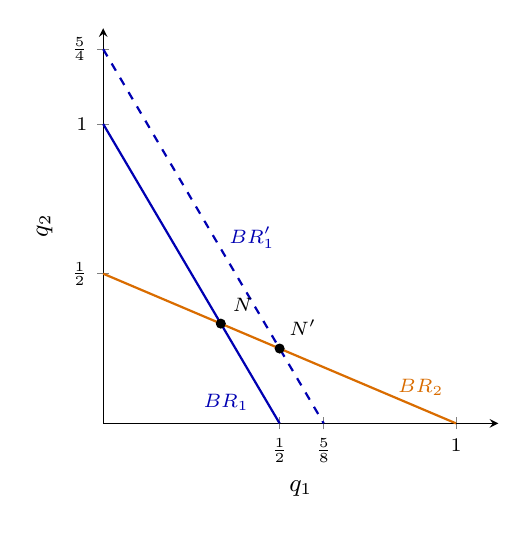
\begin{tikzpicture}
\begin{axis}[
  width=6.6cm, height=6.6cm,
  xmin=0, xmax=1.12, ymin=0, ymax=1.32,
  axis lines=left,
  xlabel={$q_1$}, ylabel={$q_2$},
  xtick={0.5,0.625,1}, xticklabels={$\frac{1}{2}$,$\frac{5}{8}$,$1$},
  ytick={0.5,1,1.25}, yticklabels={$\frac{1}{2}$,$1$,$\frac{5}{4}$},
  tick label style={font=\scriptsize}, label style={font=\small},
  clip=false]
  \addplot[blue!70!black, thick, domain=0:0.5, samples=2] {1-2*x};
  \addplot[blue!70!black, thick, dashed, domain=0:0.625, samples=2] {1.25-2*x};
  \addplot[orange!85!black, thick, domain=0:1, samples=2] {(1-x)/2};
  \addplot[only marks, mark=*, mark size=1.6pt] coordinates {(0.3333,0.3333) (0.5,0.25)};
  \node[font=\scriptsize, anchor=south west] at (axis cs:0.34,0.34) {$N$};
  \node[font=\scriptsize, anchor=south west] at (axis cs:0.5,0.26) {$N'$};
  \node[font=\scriptsize, anchor=east, blue!70!black] at (axis cs:0.44,0.07) {$BR_1$};
  \node[font=\scriptsize, anchor=west, blue!70!black] at (axis cs:0.33,0.62) {$BR_1'$};
  \node[font=\scriptsize, anchor=south, orange!85!black] at (axis cs:0.9,0.06) {$BR_2$};
\end{axis}
\end{tikzpicture}
\caption{Cournot: strategic substitutes}
\end{subfigure}\hfill
\begin{subfigure}[t]{0.48\textwidth}
\centering
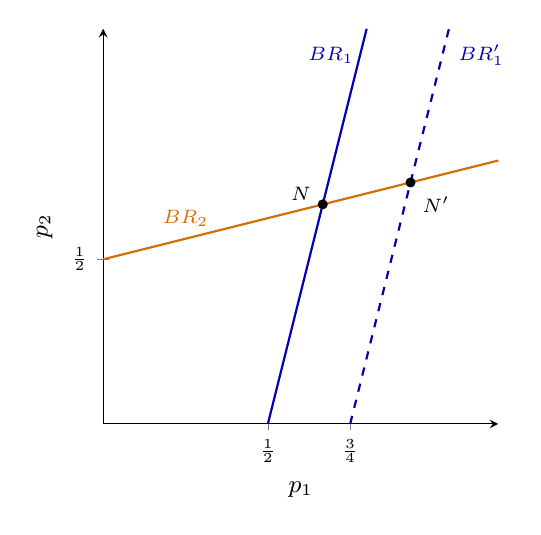
\begin{tikzpicture}
\begin{axis}[
  width=6.6cm, height=6.6cm,
  xmin=0, xmax=1.2, ymin=0, ymax=1.2,
  axis lines=left,
  xlabel={$p_1$}, ylabel={$p_2$},
  xtick={0.5,0.75}, xticklabels={$\frac{1}{2}$,$\frac{3}{4}$},
  ytick={0.5}, yticklabels={$\frac{1}{2}$},
  tick label style={font=\scriptsize}, label style={font=\small},
  clip=false]
  \addplot[blue!70!black, thick, domain=0.5:0.8, samples=2] {4*(x-0.5)};
  \addplot[blue!70!black, thick, dashed, domain=0.75:1.05, samples=2] {4*(x-0.75)};
  \addplot[orange!85!black, thick, domain=0:1.2, samples=2] {0.5+x/4};
  \addplot[only marks, mark=*, mark size=1.6pt] coordinates {(0.6667,0.6667) (0.9333,0.7333)};
  \node[font=\scriptsize, anchor=east] at (axis cs:0.66,0.70) {$N$};
  \node[font=\scriptsize, anchor=north west] at (axis cs:0.94,0.72) {$N'$};
  \node[font=\scriptsize, anchor=east, blue!70!black] at (axis cs:0.79,1.12) {$BR_1$};
  \node[font=\scriptsize, anchor=west, blue!70!black] at (axis cs:1.05,1.12) {$BR_1'$};
  \node[font=\scriptsize, anchor=south, orange!85!black] at (axis cs:0.25,0.57) {$BR_2$};
\end{axis}
\end{tikzpicture}
\caption{Differentiated Bertrand: strategic complements}
\end{subfigure}
\caption{Reaction curves under strategic substitutes and complements. Panel (a): Cournot duopoly with inverse
demand $P = a_0 - Q$ and $a_0 - c = 1$, so $BR_i(q_j) = \frac{1 - q_j}{2}$ and the equilibrium is
$N = (\frac{1}{3}, \frac{1}{3})$. A cost reduction of $\frac{1}{4}$ for firm 1 shifts its curve to
$BR_1'(q_2) = \frac{5}{8} - \frac{q_2}{2}$, and the new equilibrium is $N' = (\frac{1}{2}, \frac{1}{4})$: firm 2
contracts. Panel (b): the demand of \citet[Section~11.2]{Tirole1988} with $b = 1$ and $d = \frac{1}{2}$,
$q_i = 1 - p_i + \frac{1}{2}p_j$, with zero cost, so
$BR_i(p_j) = \frac{1}{2} + \frac{1}{4}p_j$ and $N = (\frac{2}{3}, \frac{2}{3})$. Raising firm 1's cost to $\frac{1}{2}$ shifts
its curve to $BR_1'(p_2) = \frac{3}{4} + \frac{1}{4}p_2$, and the new equilibrium is
$N' = (\frac{14}{15}, \frac{11}{15})$: both prices rise.}
\label{fig:B-reaction}
\end{figure}

\subsection{Supermodular games}\label{sec:B-supermodular-games}

Games with strategic complements have a lattice structure that delivers existence, computation and comparative
statics with no concavity and no differentiability. The fixed-point theorem behind them is due to Tarski.

\begin{theorem}[Tarski]\label{thm:B-tarski}
Let $\mathcal{X}$ be a complete lattice and $T : \mathcal{X} \to \mathcal{X}$ a nondecreasing map, that is, $x \leq x'$ implies
$T(x) \leq T(x')$. Then $T$ has a fixed point. Its largest fixed point is $\sup\{x \in \mathcal{X} : x \leq T(x)\}$, and the set
of fixed points is itself a complete lattice \citep{Tarski1955}.
\end{theorem}

\begin{proof}[Proof of existence]
Let $\mathcal{S} = \{x \in \mathcal{X} : x \leq T(x)\}$. It is nonempty because it contains $\inf\mathcal{X}$. Let
$\bar x = \sup\mathcal{S}$. For any $x \in \mathcal{S}$, $x \leq \bar x$, so $x \leq T(x) \leq T(\bar x)$. Thus $T(\bar x)$ is an
upper bound of $\mathcal{S}$, and $\bar x \leq T(\bar x)$. Applying $T$ gives $T(\bar x) \leq T(T(\bar x))$, so
$T(\bar x) \in \mathcal{S}$ and $T(\bar x) \leq \bar x$. Hence $T(\bar x) = \bar x$. Every fixed point lies in $\mathcal{S}$,
so $\bar x$ is the largest.
\end{proof}

Unlike Brouwer's and Kakutani's theorems, Tarski's theorem needs no continuity and no convexity. Monotonicity
does all the work.

\begin{definition}[Supermodular game]\label{def:B-smgame}
A game with players $i = 1, \dots, N$, strategy sets $X_i$ and payoffs $u_i(x_i, x_{-i})$ is \emph{supermodular} if
three conditions hold. Each $X_i$ is a compact product of intervals in some $\R^{k_i}$. Each $u_i$ is upper
semicontinuous in $x_i$ and continuous in $x_{-i}$. Each $u_i$ is supermodular in $x_i$ and has increasing differences
in $(x_i, x_{-i})$.
\end{definition}

Supermodularity in own strategy is automatic when each $x_i$ is a scalar. Increasing differences in
$(x_i, x_{-i})$ is strategic complementarity.

\begin{theorem}[Supermodular games]\label{thm:B-smgames}
In a supermodular game the following hold.
\begin{enumerate}[label=(\roman*)]
  \item The set of pure-strategy Nash equilibria is nonempty. It has a largest element $\bar x$ and a smallest
  element $\underline x$.
  \item Best-response iteration from the largest strategy profile, choosing the largest best response at each
  step, decreases monotonically to $\bar x$. Iteration from the smallest profile increases to $\underline x$.
  \item Suppose each $u_i(x_i, x_{-i}; a)$ has increasing differences in $(x_i, a)$ for a parameter $a$. Then $\bar x(a)$
  and $\underline x(a)$ are nondecreasing in $a$.
  \item Every strategy that survives iterated elimination of strictly dominated strategies lies between
  $\underline x$ and $\bar x$. A game with a unique equilibrium is therefore dominance solvable, and adaptive dynamics
  converge to it.
\end{enumerate}
\end{theorem}

\begin{proof}[Proof sketch]
(i) By \cref{thm:B-topkis}, applied with $x_{-i}$ as the parameter, player $i$'s set of best responses has a largest
element $\bar b_i(x_{-i})$, nondecreasing in $x_{-i}$. Upper semicontinuity and compactness ensure the set is
nonempty and has a largest element. The map $\bar b = (\bar b_1, \dots, \bar b_N)$ is a nondecreasing self-map of the
complete lattice $\prod_iX_i$. By \cref{thm:B-tarski} it has a largest fixed point $\bar x$, which is an equilibrium. If
$x^*$ is any equilibrium, then $x_i^* \leq \bar b_i(x_{-i}^*)$ for every $i$, so $x^* \leq \bar b(x^*)$ and $x^* \leq \bar x$ by the
characterization in \cref{thm:B-tarski}. The smallest equilibrium is symmetric.

(ii) Let $x^{(0)} = \sup\prod_iX_i$ and $x^{(h+1)} = \bar b(x^{(h)})$. Trivially $x^{(1)} \leq x^{(0)}$, and monotonicity of
$\bar b$ gives $x^{(h+1)} \leq x^{(h)}$ by induction. Similarly $\bar x \leq x^{(0)}$ implies $\bar x = \bar b(\bar x) \leq x^{(h)}$
for all $h$. The decreasing sequence converges, and continuity of payoffs makes its limit an equilibrium. The
limit is at least $\bar x$, so it equals $\bar x$.

(iii) If $a' \geq a$, then $\bar b(x; a') \geq \bar b(x; a)$ for every $x$ by \cref{thm:B-topkis}. Any $x$ with $x \leq \bar b(x; a)$
then satisfies $x \leq \bar b(x; a')$. The set whose supremum defines the largest fixed point grows with $a$, so its
supremum rises. Part (iv) is due to \citet{MilgromRoberts1990}.
\end{proof}

The results are due to \citet{Topkis1979}, \citet{Vives1990} and \citet{MilgromRoberts1990}, and \citet{Vives1999}
develops the oligopoly applications. When payoffs are positive, the theorem applies to a game with
log-supermodular payoffs after replacing $u_i$ by $\ln u_i$, because the transformation leaves best responses unchanged.

\begin{example}[A cost increase raises all logit prices]\label{ex:B-logit-cost}
Consider the single-product logit pricing game, and fix an interval of firm 1's costs
$[\underline{mc}_1, \overline{mc}_1]$ of length below $\frac{1}{\alpha}$. Every best response carries a markup
$\frac{1 + W_0(z_j)}{\alpha} > \frac{1}{\alpha}$ (\cref{prop:B-logit-br}). Since $\Lambda_{-j} \geq 1$, we have
$z_j \leq e^{v_j - 1}$, so best responses are also bounded above, uniformly over the interval of costs. Let $\bar p$
be such a bound. We restrict firm 1 to $[\underline{mc}_1 + \frac{1}{\alpha}, \bar p]$ and each firm $j \neq 1$ to
$[mc_j + \frac{1}{\alpha}, \bar p]$. These sets contain every best response, so the restriction leaves the equilibria
unchanged. The sets do not move with $mc_1$. On them every price exceeds marginal cost, so profits are positive and
log profits are finite. By \cref{ex:B-strategic-examples}(c), log profits have increasing differences in every pair of
prices. With firm 1's marginal cost as the parameter,
\[
  \frac{\partial^2\ln\pi_1}{\partial p_1\,\partial mc_1} = \frac{\partial}{\partial mc_1}\left[\frac{1}{p_1 - mc_1}\right] = \frac{1}{(p_1 - mc_1)^2} > 0,
\]
while the log profits of the other firms do not depend on $mc_1$. By \cref{thm:B-smgames}(iii) the extremal
equilibria are nondecreasing in $mc_1$ on the interval. Any two costs are linked by a chain of overlapping intervals
of this kind, so the conclusion holds for any two costs. The equilibrium is unique (\cref{sec:B-caplin-nalebuff}), so every firm's
equilibrium price is nondecreasing in firm 1's cost. This is the last property in Caplin and Nalebuff's list.
\end{example}

Two further applications follow the same pattern. First, a merger of two price-setting firms with substitute
products adds the partner's profit to each merging firm's objective. With weight $a \in [0, 1]$ on the partner's
profit, the objective $\pi_1 + a\pi_2$ has $\frac{\partial^2(\pi_1 + a\pi_2)}{\partial p_1\,\partial a} = \frac{\partial\pi_2}{\partial p_1} = (p_2 - mc_2)\frac{\partial q_2}{\partial p_1} \geq 0$
whenever $p_2 \geq mc_2$. When the post-merger game remains supermodular, as with linear demand, all equilibrium
prices rise, the merging firms' and the outsiders' alike \citep{DeneckereDavidson1985}. \Cref{ch:mergers} develops
merger simulation. Second, with strategic complements a firm's best deviation from a collusive price profile
lies above the static Nash price, because best responses slope up. The slope of best responses therefore
governs the gain from deviating (\cref{ch:collusion-theory}).

\subsection{Stochastic orders}\label{sec:B-stochastic-orders}

Probability brings its own orders. Let $X_A$ and $X_B$ have CDFs $F_A$ and $F_B$ with densities $f_A$ and $f_B$ that are
positive on a common support $(\underline x, \bar x)$.

\begin{definition}[Stochastic orders]\label{def:B-orders}
\leavevmode
\begin{enumerate}[label=(\roman*)]
  \item $X_B$ dominates $X_A$ in the \emph{first-order stochastic dominance} order, $X_B \geq_{\mathrm{FOSD}} X_A$, if
  $F_B(x) \leq F_A(x)$ for all $x$.
  \item $X_B \geq_{\mathrm{hr}} X_A$ in the \emph{hazard rate order} if $\frac{f_B(x)}{1 - F_B(x)} \leq \frac{f_A(x)}{1 - F_A(x)}$
  for all $x$.
  \item $X_B \geq_{\mathrm{rh}} X_A$ in the \emph{reverse hazard rate order} if $\frac{f_B(x)}{F_B(x)} \geq \frac{f_A(x)}{F_A(x)}$
  for all $x$.
  \item $X_B \geq_{\mathrm{lr}} X_A$ in the \emph{likelihood ratio order} if $\frac{f_B(x)}{f_A(x)}$ is nondecreasing in $x$.
  This is the \emph{monotone likelihood ratio property} (MLRP).
\end{enumerate}
\end{definition}

\Cref{def:14-rhr} defines the same four orders for the values of strong and weak bidders. The higher variable
has the lower hazard rate, because it is less likely to stop just after any level. It has the
higher reverse hazard rate, because it is more concentrated near the top of any truncation from above.

\begin{proposition}[The chain of stochastic orders]\label{prop:B-orders-chain}
The likelihood ratio order implies both the hazard rate order and the reverse hazard rate order, and each of these
implies first-order stochastic dominance:
\[
  \geq_{\mathrm{lr}} \;\implies\; \geq_{\mathrm{hr}} \text{ and } \geq_{\mathrm{rh}}, \qquad
  \geq_{\mathrm{hr}} \;\implies\; \geq_{\mathrm{FOSD}}, \qquad
  \geq_{\mathrm{rh}} \;\implies\; \geq_{\mathrm{FOSD}}.
\]
\end{proposition}

\begin{proof}
Assume the MLRP and fix $x$. For every $t \leq x$, $\frac{f_B(t)}{f_A(t)} \leq \frac{f_B(x)}{f_A(x)}$, that is,
\[
  f_B(t)f_A(x) \leq f_A(t)f_B(x).
\]
Integrating over $t \in (\underline x, x]$ gives $F_B(x)f_A(x) \leq F_A(x)f_B(x)$, which rearranges to
$\frac{f_B(x)}{F_B(x)} \geq \frac{f_A(x)}{F_A(x)}$, the reverse hazard rate order. For $t \geq x$ the inequality reverses,
$f_B(t)f_A(x) \geq f_A(t)f_B(x)$. Integrating over $t \in [x, \bar x)$ gives
$(1 - F_B(x))f_A(x) \geq (1 - F_A(x))f_B(x)$, which rearranges to the hazard rate order.

The reverse hazard rate order implies dominance by \cref{prop:B-rh-fosd}. For the hazard rate order, use
$\frac{f}{1 - F} = -\frac{\dd}{\dd x}\ln(1 - F)$. The hypothesis says
\[
  \frac{\dd}{\dd x}\ln\frac{1 - F_B(x)}{1 - F_A(x)} = \frac{f_A(x)}{1 - F_A(x)} - \frac{f_B(x)}{1 - F_B(x)} \geq 0.
\]
The ratio $\frac{1 - F_B}{1 - F_A}$ is nondecreasing and tends to one at $\underline x$. Hence it is at least one, and
$F_B(x) \leq F_A(x)$.
\end{proof}

None of the converse implications holds in general \citep{ShakedShanthikumar2007}. First-order dominance has a
useful characterization through expectations.

\begin{proposition}[Dominance and expectations]\label{prop:B-fosd-expectations}
$X_B \geq_{\mathrm{FOSD}} X_A$ if and only if $\E[\varphi(X_B)] \geq \E[\varphi(X_A)]$ for every nondecreasing function $\varphi$ for which
both expectations exist.
\end{proposition}

\begin{proof}
For the ``if'' direction, take $\varphi(x) = \indic\{x > t\}$. Then $\E[\varphi(X)] = 1 - F(t)$, so $1 - F_B(t) \geq 1 - F_A(t)$ for
every $t$. For the ``only if'' direction, let $U \sim U[0, 1]$ and define $\tilde X_A = F_A^{-1}(U)$ and $\tilde X_B = F_B^{-1}(U)$
with the generalized inverses $F^{-1}(u) = \inf\{x : F(x) \geq u\}$. By \cref{lem:B-pit}, $\tilde X_A$ and $\tilde X_B$ have the
distributions of $X_A$ and $X_B$. If $F_B \leq F_A$, then $\{x : F_B(x) \geq u\} \subseteq \{x : F_A(x) \geq u\}$, so the infimum over the
smaller set is larger and $\tilde X_B \geq \tilde X_A$ pointwise. Then $\varphi(\tilde X_B) \geq \varphi(\tilde X_A)$ for every realization, and
taking expectations completes the proof.
\end{proof}

A family of conditional distributions $F(\cdot \mid z)$ is \emph{stochastically increasing} in $z$ if
$F(\cdot \mid z') \leq F(\cdot \mid z)$ whenever $z' > z$. By \cref{prop:B-fosd-expectations}, $\E[\varphi(X) \mid Z = z]$ is then
nondecreasing in $z$ for every nondecreasing $\varphi$. Affiliation, to which we turn, is the multivariate
condition that delivers such monotonicity.

\subsection{Affiliation}\label{sec:B-affiliation}

Affiliation is log-supermodularity of a joint density. It is the form of positive dependence under which
\citet{MilgromWeber1982} develop the theory of auctions with interdependent values (\cref{ch:auction-theory}).

\begin{definition}[Affiliation]\label{def:B-affiliation}
A random vector $Z = (Z_1, \dots, Z_k)$ with joint density $f$ is \emph{affiliated} if, for all $z, z' \in \R^k$,
\begin{equation}\label{eq:B-affil}
  f(z \vee z')\,f(z \wedge z') \geq f(z)\,f(z')
\end{equation}
\citep[eq.~(2), p.~1098]{MilgromWeber1982}.
\end{definition}

The same definition appears in \citet[footnote 9]{AtheyHaile2007} and as \cref{def:14-affiliation}. Inequality
\eqref{eq:B-affil} is also called the FKG inequality \citep{FortuinKasteleynGinibre1971} and the MTP$_2$ property,
multivariate total positivity of order two \citep{KarlinRinott1980}. Where $f > 0$, taking logs shows that
affiliation is exactly log-supermodularity of the density. Roughly, large values of some of the variables make
large values of the others more likely \citep[p.~1098]{MilgromWeber1982}. Independent variables satisfy
\eqref{eq:B-affil} with equality, because both sides contain the same marginal factors.

\begin{figure}[htbp]
\centering
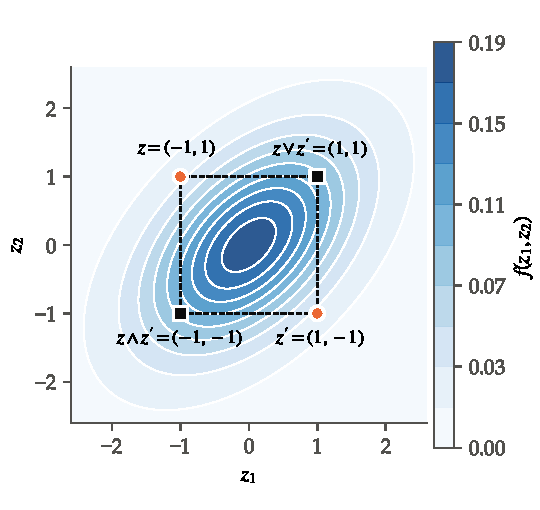
\includegraphics[width=0.56\textwidth]{figures/appB/affiliation.pdf}
\caption{The affiliation inequality for the standard bivariate normal density with correlation $\frac{1}{2}$. The
unordered points $z = (-1, 1)$ and $z' = (1, -1)$ (circles) have join $z \vee z' = (1, 1)$ and meet $z \wedge z' = (-1, -1)$
(squares). The density is $0.09435$ at the join and the meet and $0.02487$ at $z$ and $z'$, so
$f(z \vee z')f(z \wedge z') = 0.00890$ exceeds $f(z)f(z') = 0.000619$, by the factor $e^{\frac{8}{3}} \approx 14.39$.}
\label{fig:B-affiliation}
\end{figure}

\begin{remark}[The general definition]\label{rem:B-affil-general}
\citet[Appendix]{MilgromWeber1982} define affiliation without densities. A set $A \subseteq \R^k$ is \emph{increasing} if its
indicator is nondecreasing, and a set $S$ is a sublattice if $z \vee z', z \wedge z' \in S$ whenever $z, z' \in S$. The variables
are \emph{associated} if $\Pr(Z \in A \cap A') \geq \Pr(Z \in A)\Pr(Z \in A')$ for all increasing sets $A$ and $A'$. They are
affiliated if they are associated conditional on every sublattice $S$ of positive probability. Their Theorem 24
shows that, for variables with a density, this is equivalent to \eqref{eq:B-affil} almost everywhere.
\end{remark}

\begin{proposition}[Characterization, \citealp{MilgromWeber1982}, Theorem 1]\label{prop:B-affil-char}
\leavevmode
\begin{enumerate}[label=(\roman*)]
  \item A strictly positive, twice continuously differentiable density $f$ on a product of intervals is affiliated if
  and only if $\frac{\partial^2\ln f}{\partial z_l\,\partial z_m} \geq 0$ for all $l \neq m$.
  \item If $f = g_1g_2$ with $g_1$ and $g_2$ nonnegative functions that satisfy \eqref{eq:B-affil}, then $f$ is affiliated.
\end{enumerate}
\end{proposition}

\Cref{prop:14-affil-char} proves both parts. Part (i) is also \cref{prop:B-smooth-supermod} applied to $\ln f$, and
\citet[p.~1098]{MilgromWeber1982} cite \citet[p.~310]{Topkis1978} for it. Part (ii) multiplies the inequalities
for $g_1$ and $g_2$, which is legitimate because all terms are nonnegative.

For two variables, affiliation is a statement about conditional densities, and it feeds directly into the chain of
stochastic orders.

\begin{proposition}[Affiliation, MLRP and dominance]\label{prop:B-affil-mlrp}
Let $(X, Z)$ have a strictly positive density $f(x, z)$ on a rectangle, with conditional density $f(x \mid z)$ and
conditional CDF $F(x \mid z)$.
\begin{enumerate}[label=(\roman*)]
  \item $(X, Z)$ is affiliated if and only if $f(x \mid z)$ has the MLRP in $z$: for $z' > z$, $\frac{f(x \mid z')}{f(x \mid z)}$ is
  nondecreasing in $x$.
  \item Let $(X, Z)$ be affiliated and $z' > z$. The conditional distribution given $z'$ dominates the one given $z$ in
  the reverse hazard rate and hazard rate orders. In particular, $\Pr(X \geq x \mid Z = z)$ is nondecreasing in $z$.
  \item If $(X, Z)$ is affiliated, then $\E[\varphi(X) \mid Z = z]$ is nondecreasing in $z$ for every nondecreasing $\varphi$.
\end{enumerate}
\end{proposition}

\begin{proof}
(i) For $x' > x$ and $z' > z$, inequality \eqref{eq:B-affil} reads $f(x', z')f(x, z) \geq f(x, z')f(x', z)$. Dividing by the
product of the marginal densities of $Z$ at $z$ and $z'$ turns joint densities into conditional ones, and dividing
again by $f(x' \mid z)f(x \mid z) > 0$ gives
$\frac{f(x' \mid z')}{f(x' \mid z)} \geq \frac{f(x \mid z')}{f(x \mid z)}$, the MLRP. Each step reverses
\citep[footnote 16]{MilgromWeber1982}. Parts (ii) and (iii) follow from part (i) by \cref{prop:B-orders-chain} and
\cref{prop:B-fosd-expectations}, applied to $X_B \sim F(\cdot \mid z')$ and $X_A \sim F(\cdot \mid z)$.
\end{proof}

Part (ii) follows from the affiliation that \citet{CampoPerrigneVuong2003} assume in their asymmetric affiliated
private values model, so that $\Pr(V_1 \geq v \mid V_2 = v_2)$ is nondecreasing in $v_2$. \Cref{ch:auction-theory}
proves the same chain in the auction notation. Milgrom and Weber derive the properties that auction theory needs
from affiliation.

\begin{proposition}[Properties of affiliated variables, \citealp{MilgromWeber1982}, Theorems 2--5]\label{prop:B-affil-properties}
Let $Z = (Z_1, \dots, Z_k)$ be affiliated.
\begin{enumerate}[label=(\roman*)]
  \item (Order statistics.) Suppose the density $f(s, x_1, \dots, x_n)$ of a common component $s$ and signals $x_i$ is
  affiliated and symmetric in $(x_2, \dots, x_n)$. Let $Y_1 \geq \dots \geq Y_{n-1}$ be the order statistics of
  $(X_2, \dots, X_n)$. Then $(S, X_1, Y_1, \dots, Y_{n-1})$ is affiliated.
  \item (Monotone transformations.) If $g_1, \dots, g_k$ are all nondecreasing or all nonincreasing, then
  $g_1(Z_1), \dots, g_k(Z_k)$ are affiliated.
  \item (Subvectors.) $Z_1, \dots, Z_{k-1}$ are affiliated.
  \item (Conditional expectations.) For any nondecreasing $H$, the function
  $h(a_1, b_1; \dots; a_k, b_k) = \E[H(Z) \mid a_1 \leq Z_1 \leq b_1, \dots, a_k \leq Z_k \leq b_k]$ is nondecreasing in all its arguments.
  In particular, $\E[H(Z) \mid Z_1 = z_1, \dots, Z_l = z_l]$ is nondecreasing in $(z_1, \dots, z_l)$.
\end{enumerate}
\end{proposition}

\begin{proof}[Proofs and sketches]
(i) The joint density of $(S, X_1, Y_1, \dots, Y_{n-1})$ is
\[
  (n - 1)!\,f(s, x_1, y_1, \dots, y_{n-1})\,\indic\{y_1 \geq y_2 \geq \dots \geq y_{n-1}\}
\]
\citep[eq.~(4), p.~1099]{MilgromWeber1982}. The set of ordered vectors is a lattice, because componentwise maxima
and minima of two decreasing sequences are decreasing. Its indicator therefore satisfies \eqref{eq:B-affil}. The
product rule of \cref{prop:B-affil-char}(ii) gives the result.

(ii) We prove the case of strictly increasing, differentiable $g_l$. By the change-of-variables formula, the density
of $W = (g_1(Z_1), \dots, g_k(Z_k))$ is
\[
  f_W(w) = f\bigl(g_1^{-1}(w_1), \dots, g_k^{-1}(w_k)\bigr)\prod_{l=1}^k\frac{1}{g_l'(g_l^{-1}(w_l))}.
\]
The map $w \mapsto (g_1^{-1}(w_1), \dots, g_k^{-1}(w_k))$ is increasing coordinate by coordinate, so it commutes with joins and
meets. The first factor therefore satisfies \eqref{eq:B-affil}. The product is a product of functions of one
coordinate each, which satisfies \eqref{eq:B-affil} with equality. \Cref{prop:B-affil-char}(ii) completes the
argument. If all $g_l$ are decreasing, joins and meets swap, and \eqref{eq:B-affil} is symmetric in them.

(iii) Write $Z = (U, W)$ with $U = (Z_1, \dots, Z_{k-1})$ and $W = Z_k$, and let $f(u, w)$ be the joint density. Fix
$u, u' \in \R^{k-1}$. We must show that the marginal $\int f(u, w)\,\dd w$ satisfies \eqref{eq:B-affil}, that is,
\[
  \int f(u \vee u', w)\,\dd w\int f(u \wedge u', w)\,\dd w \geq \int f(u, w)\,\dd w\int f(u', w)\,\dd w.
\]
Write each product as a double integral over $(w, w')$ and fold the region $w > w'$ onto $w < w'$. For $w < w'$ define
\begin{align*}
  \Theta_1 &= f(u \vee u', w)f(u \wedge u', w'), & \Theta_2 &= f(u \vee u', w')f(u \wedge u', w),\\
  \Xi_1 &= f(u, w)f(u', w'), & \Xi_2 &= f(u, w')f(u', w).
\end{align*}
The left side is the integral of $\Theta_1 + \Theta_2$ and the right side the integral of $\Xi_1 + \Xi_2$ over $w < w'$, so it
suffices to show $\Theta_1 + \Theta_2 \geq \Xi_1 + \Xi_2$ pointwise. Affiliation of $f$ gives $\Theta_2 \geq \Xi_1$ and $\Theta_2 \geq \Xi_2$,
because in both cases the join of the two arguments is $(u \vee u', w')$ and the meet is $(u \wedge u', w)$. Affiliation in $u$
at fixed $w$ and at fixed $w'$ gives, after multiplying, $\Theta_1\Theta_2 \geq \Xi_1\Xi_2$. Now
$(\Theta_2 - \Xi_1)(\Theta_2 - \Xi_2) \geq 0$ expands to
\[
  \Theta_2(\Xi_1 + \Xi_2) \leq \Theta_2^2 + \Xi_1\Xi_2 \leq \Theta_2^2 + \Theta_1\Theta_2.
\]
Dividing by $\Theta_2 > 0$ gives the claim. If $\Theta_2 = 0$, then $\Xi_1 = \Xi_2 = 0$ and the claim is trivial. This is the
simplest case of the composition results of \citet{KarlinRinott1980}.

(iv) We prove the bivariate case $k = 2$, $l = 1$. Write $\E[H(Z_1, Z_2) \mid Z_1 = z_1] = \E[H(z_1, Z_2) \mid Z_1 = z_1]$. Raising
$z_1$ raises the integrand $H(z_1, \cdot)$ pointwise, and it shifts the conditional distribution of $Z_2$ up in the sense of
first-order dominance (\cref{prop:B-affil-mlrp}). By \cref{prop:B-fosd-expectations} both effects raise the
conditional expectation. \citet[Appendix]{MilgromWeber1982} derive the general statement from the conditional
covariance inequality below.
\end{proof}

Affiliation implies a covariance inequality that is often easier to use than the density condition.

\begin{theorem}[Association, \citealp{MilgromWeber1982}, Theorems 22--23]\label{thm:B-association}
If $Z$ is affiliated, then for every pair of nondecreasing functions $g$ and $h$ and every sublattice $S$ of positive
probability,
\[
  \E[g(Z)h(Z) \mid S] \geq \E[g(Z) \mid S]\,\E[h(Z) \mid S].
\]
With $S = \R^k$, affiliated variables are \emph{associated}: $\Cov(g(Z), h(Z)) \geq 0$. Moreover,
$\E[g(Z) \mid A] \geq \E[g(Z)] \geq \E[g(Z) \mid A^c]$ for every increasing set $A$ of positive probability.
\end{theorem}

\begin{proof}[Proof for one variable]
Let $k = 1$ and let $Z'$ be an independent copy of $Z$. Because $g$ and $h$ are both nondecreasing, $g(Z) - g(Z')$ and
$h(Z) - h(Z')$ have the same sign, so
\[
  0 \leq \E\bigl[(g(Z) - g(Z'))(h(Z) - h(Z'))\bigr] = 2\E[g(Z)h(Z)] - 2\E[g(Z)]\E[h(Z)].
\]
This is Chebyshev's covariance inequality. For general $k$, the inequality for indicators of increasing sets is
association, which is part of Milgrom and Weber's general definition of affiliation (\cref{rem:B-affil-general}).
Their Theorem 24 shows that a density satisfying \eqref{eq:B-affil} is affiliated in that sense. The step functions
$g_m(z) = \frac{1}{m}\sum_{i \geq 1}\indic\{g(z) > \frac{i}{m}\}$ are sums of indicators of increasing sets and approximate a
nonnegative nondecreasing $g$, which extends the inequality from indicators to functions
\citep[Theorems 22--23]{MilgromWeber1982}. Conditioning on a sublattice $S$ multiplies the density by the indicator
of $S$, which satisfies \eqref{eq:B-affil}, so the conditional density is again affiliated.
\end{proof}

Taking $g$ and $h$ to be coordinate functions shows that affiliated variables are nonnegatively correlated. The
converse fails badly, as the examples show.

\begin{example}[Affiliated and non-affiliated densities]\label{ex:B-affil-examples}
\leavevmode
\begin{enumerate}[label=(\alph*)]
  \item \emph{Independence.} A product of marginal densities satisfies \eqref{eq:B-affil} with equality.
  \item \emph{Normal vectors.} Let $Z \sim N(\mu, \Sigma)$. Then $\ln f(z) = \text{const} - \frac{1}{2}(z - \mu)^\T\Sigma^{-1}(z - \mu)$, and
  $\frac{\partial^2\ln f}{\partial z_l\,\partial z_m} = -(\Sigma^{-1})_{lm}$. By \cref{prop:B-affil-char}(i), $Z$ is affiliated if and only if
  every off-diagonal element of the precision matrix $\Sigma^{-1}$ is nonpositive. In the bivariate case with standard
  deviations $\sigma_1$, $\sigma_2$ and correlation $\rho_{12}$ (written with a subscript to distinguish it from
  pass-through),
  \[
    \ln f = \text{const} - \frac{1}{2(1 - \rho_{12}^2)}\left[\frac{(z_1 - \mu_1)^2}{\sigma_1^2} - \frac{2\rho_{12}(z_1 - \mu_1)(z_2 - \mu_2)}{\sigma_1\sigma_2} + \frac{(z_2 - \mu_2)^2}{\sigma_2^2}\right],
  \]
  so $\frac{\partial^2\ln f}{\partial z_1\,\partial z_2} = \frac{\rho_{12}}{(1 - \rho_{12}^2)\sigma_1\sigma_2}$. A bivariate normal vector is affiliated
  if and only if $\rho_{12} \geq 0$. With three or more variables, nonnegative correlations do not suffice. The
  covariance matrix with unit variances and correlations $\Corr(Z_1, Z_2) = \Corr(Z_1, Z_3) = \frac{1}{2}$ and
  $\Corr(Z_2, Z_3) = 0$ is positive definite, but its inverse has $(\Sigma^{-1})_{23} = \frac{1}{2} > 0$. Conditional on $Z_1$, the
  variables $Z_2$ and $Z_3$ are negatively related, and the vector is not affiliated.
  \item \emph{Farlie-Gumbel-Morgenstern density.} On $[0, 1]^2$ let $c(z_1, z_2) = 1 + \vartheta(1 - 2z_1)(1 - 2z_2)$ with
  $|\vartheta| \leq 1$. It integrates to one, has uniform marginals, and $\Cov(Z_1, Z_2) = \frac{\vartheta}{36}$, so
  $\Corr(Z_1, Z_2) = \frac{\vartheta}{3}$. Its partial derivatives are $c_1 = -2\vartheta(1 - 2z_2)$, $c_2 = -2\vartheta(1 - 2z_1)$
  and $c_{12} = 4\vartheta$. Hence
  \[
    \frac{\partial^2\ln c}{\partial z_1\,\partial z_2} = \frac{c\,c_{12} - c_1c_2}{c^2}
    = \frac{4\vartheta\bigl[1 + \vartheta(1 - 2z_1)(1 - 2z_2)\bigr] - 4\vartheta^2(1 - 2z_1)(1 - 2z_2)}{c^2} = \frac{4\vartheta}{c^2}.
  \]
  The density is affiliated if and only if $\vartheta \geq 0$.
  \item \emph{Mineral rights.} Let the common value $V$ have density $h$, and let signals be $S_i = V + \epsilon_i$ with
  $\epsilon_1, \dots, \epsilon_n$ i.i.d., independent of $V$, with a log-concave density $f_\epsilon$. The conditional density of a
  signal is $f_\epsilon(s - v)$. For $v' > v$, write $t = s - v$ and $d = v' - v > 0$. Then
  \[
    \ln\frac{f_\epsilon(s - v')}{f_\epsilon(s - v)} = \ln f_\epsilon(t - d) - \ln f_\epsilon(t),
  \]
  which is nondecreasing in $t$, and hence in $s$, because the increments of the concave function $\ln f_\epsilon$ shrink as its
  argument grows. The MLRP holds. Each factor $f_\epsilon(s_i - v)$ of the joint density
  $h(v)\prod_{i=1}^n f_\epsilon(s_i - v)$ satisfies \eqref{eq:B-affil} in $(v, s_i)$, and therefore on the whole vector, since
  joins and meets act coordinate by coordinate. By \cref{prop:B-affil-char}(ii), $(V, S_1, \dots, S_n)$ is affiliated
  \citep[p.~1099]{MilgromWeber1982}. Normal, logistic and Gumbel noise all qualify (\cref{tab:B-logconcave}).
\end{enumerate}
\end{example}

\Cref{fig:B-affiliation} illustrates \eqref{eq:B-affil} for a bivariate normal density with correlation
$\frac{1}{2}$. The points $z = (-1, 1)$ and $z' = (1, -1)$ are unordered, and their join $(1, 1)$ and meet $(-1, -1)$ lie
along the direction of positive dependence, where the density is higher.

In auction theory these tools combine as follows. By \cref{prop:B-affil-properties}(i) and (iv), the expected value
$\E[V_1 \mid X_1 = x, Y_1 = y]$ is nondecreasing in both arguments, which makes symmetric equilibrium bids increasing.
By part (iv) with the upper bound on $Y_1$ lowered, $\E[V_1 \mid X_1 = x, Y_1 < x] \leq \E[V_1 \mid X_1 = x]$, which is the winner's
curse. \Cref{ch:auction-theory} develops both, and \cref{ch:auction-empirics} uses affiliation in the
identification of affiliated private values.

The first-order condition of a symmetric first-price auction with affiliated private values shows where
the conditional distributions enter. Let $B_1$ be the highest bid among bidder 1's rivals. Let
$G_{B_1|b_1}$ and $g_{B_1|b_1}$ be its distribution and density conditional on bidder 1's own bid.
\citet[eq.~4, p.~175]{LiPerrigneVuong2002} show that the equilibrium condition is equivalent to
\begin{equation*}
v = b + \frac{G_{B_1|b_1}(b \mid b)}{g_{B_1|b_1}(b \mid b)} .
\end{equation*}
Each value is therefore a known function of its bid and of the joint distribution of bids, which the data
reveal \citep[Section~3.1, eq.~3.1]{AtheyHaile2007}. Under independence the conditioning on $b_1$ drops out.
Under affiliation it stays, because a high own bid signals high rival bids. Bids inherit affiliation from
values, since the equilibrium bid function is increasing (\cref{prop:B-affil-properties}(ii)).
\citet[Proposition~1, p.~175]{LiPerrigneVuong2002} characterize the bid distributions that such a model can
generate. A distribution qualifies if and only if it is symmetric and affiliated and the right side above is
strictly increasing in $b$.
